\documentclass{article}
\usepackage[T1]{fontenc}
\usepackage{lmodern}
\usepackage{graphicx}
\usepackage{amsmath,amssymb}
\usepackage[a4paper,margin=2cm]{geometry}
\usepackage[absolute,overlay]{textpos}
\setlength{\TPHorizModule}{1mm}
\setlength{\TPVertModule}{1mm}
\usepackage[indonesian]{babel}
\usepackage{hyperref}
\setlength{\emergencystretch}{2em}
\title{08-Block-Cipher-Bagian1-(2026)}
\author{pdf\_ppt\_to\_latex}
\date{}

\begin{document}

% --- unit llm 1 ---
% === Halaman 1 (llm) ===

\begin{center}
\textbf{IF4020 Kriptografi}\\[1cm]
\Huge\textcolor{red}{08 -- Block Cipher}\\[0.5cm]
\Large\textcolor{red}{(Bagian 1)}\\[1cm]
\large\textbf{Oleh: Rinaldi M}\\[1cm]
Program Studi Teknik Informatika \\
Sekolah Teknik Elektro dan Informatika \\
Institut Teknologi Bandung \\
2026
\end{center}

\newpage

% --- unit llm 2 ---
% === Halaman 2 (llm) ===

\section*{Cipher Blok (Block Cipher)}

\begin{itemize}
    \item Berbeda dengan \textit{cipher}alir, pada \textit{cipher} blok plainteks dibagi menjadi blok-blok bit dengan panjang sama. Ukuran blok yang umum adalah 64 bit, 128 bit, 256 bit, dsb.
    \item Panjang blok cipherteks = panjang blok plainteks.
    \item Enkripsi dilakukan pada setiap blok plainteks dengan menggunakan bit-bit kunci
    \item Panjang kunci eksternal (yang diberikan oleh pengguna) tidak harus sama dengan panjang blok plainteks. Pada beberapa \textit{cipher} blok, panjang kunci = panjang blok, tetapi pada \textit{cipher} blok yang lain tidak sama.
\end{itemize}

\newpage

% --- unit llm 3 ---
% === Halaman 3 (llm) ===

\vspace{198.99mm}

\textcolor{red}{Blok plainteks berukuran $n$ bit:}
\[ P = (p_1, p_2, ..., p_n), p_i \in \{0, 1\} \]
\vspace{5mm}
\textcolor{red}{Blok cipherteks berukuran $n$ bit:}
\[ C = (c_1, c_2, ..., c_n), c_i \in \{0, 1\} \]

% deskripsi: Diagram proses enkripsi yang menunjukkan Blok plainteks P dan Kunci K masuk ke fungsi Enkripsi E untuk menghasilkan Blok cipherteks C.
% bbox normalisasi: [0.0600, 0.1080, 0.9400, 0.9120]
\begin{textblock*}{184.80mm}(12.60mm,32.08mm)
\noindent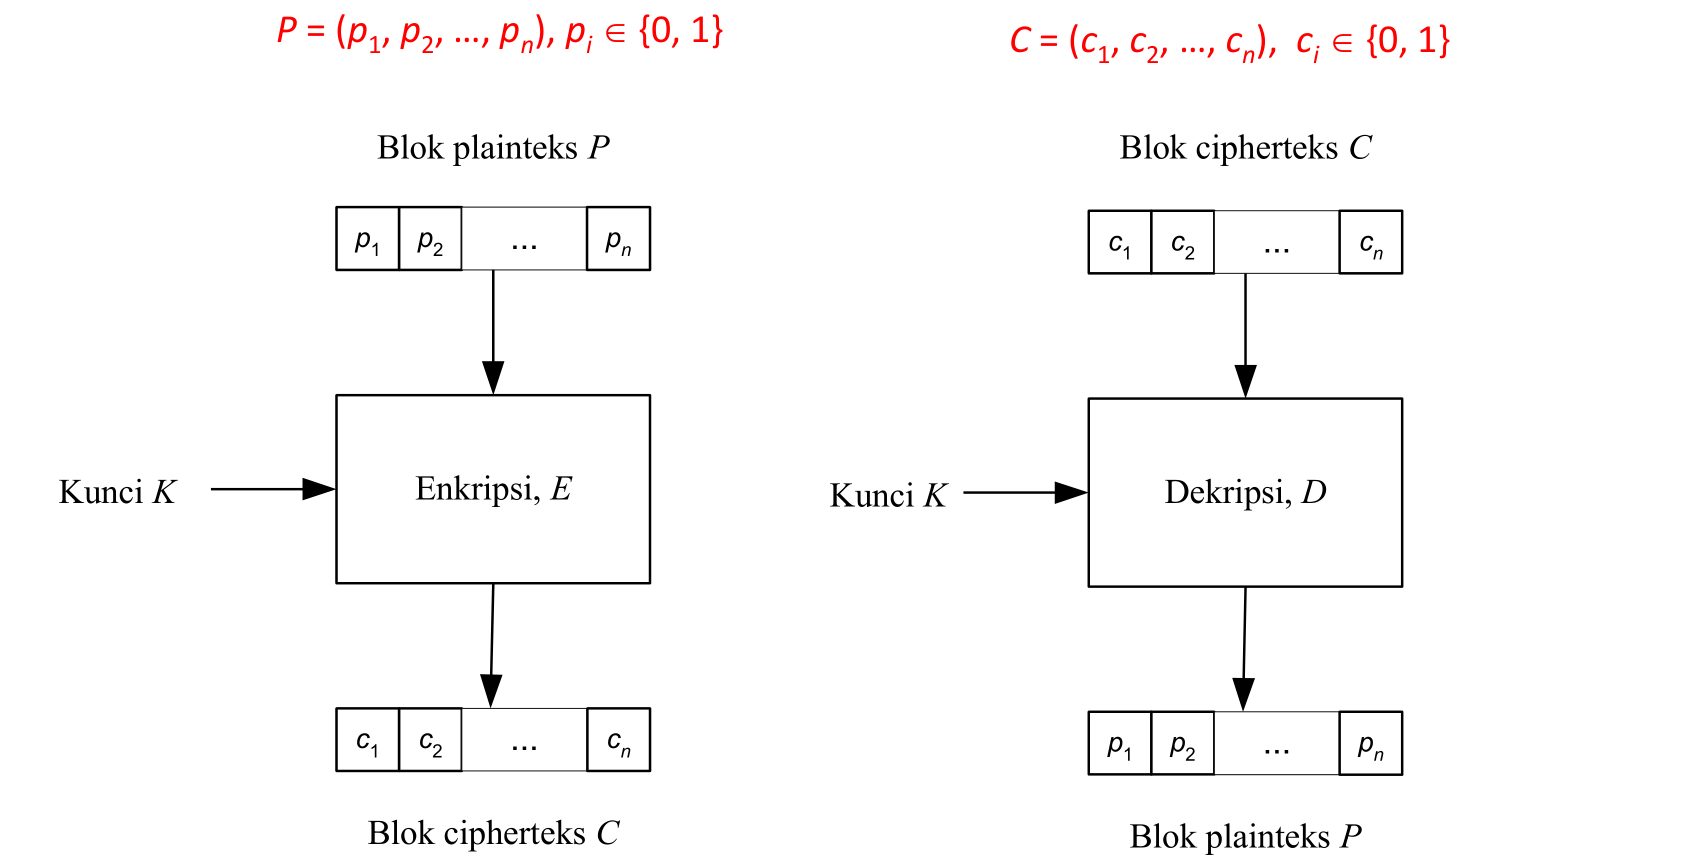
\includegraphics[width=184.80mm,height=238.79mm]{images/llm/page_003_img_01.png}%
\end{textblock*}

% deskripsi: Diagram proses dekripsi yang menunjukkan Blok cipherteks C dan Kunci K masuk ke fungsi Dekripsi D untuk menghasilkan kembali Blok plainteks P.
% bbox normalisasi: [0.4900, 0.2200, 0.8000, 0.8900]
\begin{textblock*}{65.10mm}(102.90mm,65.34mm)
\noindent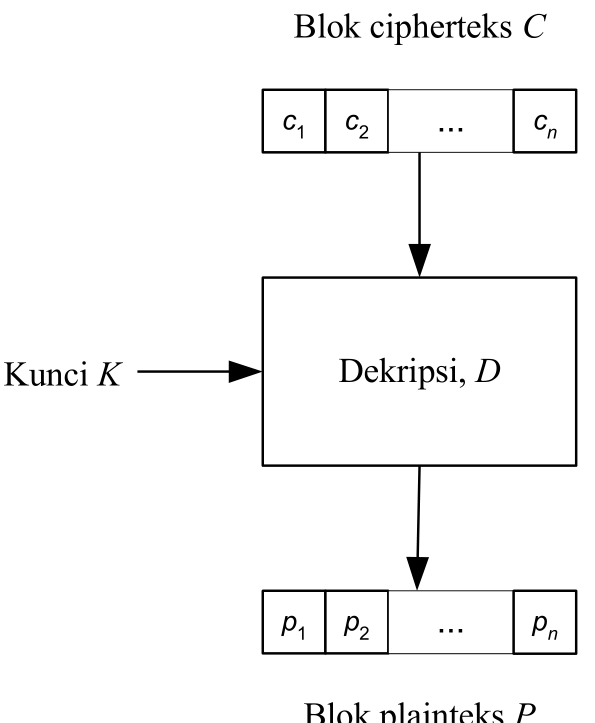
\includegraphics[width=65.10mm,height=198.99mm]{images/llm/page_003_img_02.png}%
\end{textblock*}

% bbox perkiraan otomatis: Diagram proses enkripsi yang menunjukkan Blok plainteks P dan Kunci K masuk ke fungsi Enkripsi E untuk menghasilkan Blok cipherteks C.

\newpage

% --- unit llm 4 ---
% === Halaman 4 (llm) ===

\begin{itemize}
    \item $E$ dan $D$ adalah fungsi enkripsi dan dekripsi dari suatu \textit{cipher} blok dengan parameter kunci $K$:
    \[ C = E_K(P) \quad \text{dan} \quad P = D_K(C) \]
    \item Dimisalkan contoh sebuah fungsi $E$ yang sederhana, tapi tidak cukup aman, sbb:
    \begin{enumerate}
        \item XOR-kan blok plainteks $P$ dengan $K$
        \item lalu geser secara \textit{wrapping} bit-bit dari hasil langkah 1 satu posisi ke kiri
    \end{enumerate}
    \[ C = E_K(P) = (P \oplus K) \ll 1 \]
    \item $D$ adalah kebalikan (\textit{invers}) dari $E$. Contoh fungsi $D$ yang sederhana adalah sbb:
    \begin{enumerate}
        \item Geser secara \textit{wrapping} bit-bit ciphertes $C$ satu posisi ke kanan
        \item Lalu XOR-kan blok hasil Langkah 1 dengan $K$
    \end{enumerate}
    \[ P = D_K(C) = (C \gg 1) \oplus K \]
\end{itemize}

\newpage

% --- unit llm 5 ---
% === Halaman 5 (llm) ===

\textbf{Contoh:} Misalkan plainteks adalah \textcolor{red}{1101110100010001000101000101}, dibagi menjadi tiga buah blok masing-masing berukuran 8 bit:

\begin{center}
\textcolor{red}{11011101} \quad \textcolor{red}{00010001} \quad \textcolor{red}{01000101} \\
P1 \qquad\qquad P2 \qquad\qquad P3
\end{center}

\vspace{5mm}

Kunci yang digunakan adalah $\text{K} = \textcolor{blue}{01010110}$

Enkripsi blok pertama, \textcolor{red}{11011101}, dengan fungsi $\text{E}$ sebagai berikut:
\begin{enumerate}
  \item $\text{P1} \oplus \text{K} = \textcolor{red}{11011101} \oplus \textcolor{blue}{01010110} = 10001011$
  \item $10001011 \ll 1 = 00010111$
\end{enumerate}

Jadi, $\text{C1} = 00010111$. Cara yang sama dilakukan untuk $\text{P2}$ dan $\text{P3}$.

Dekripsi blok cipherteks pertama, $00010111$, dengan fungsi $\text{D}$ sebagai berikut:
\begin{enumerate}
  \item $00010111 \gg 1 = 10001011$
  \item $10001011 \oplus \text{K} = 10001011 \oplus \textcolor{blue}{01010110} = 11011101 = \text{P1}$
\end{enumerate}

\newpage

% --- unit llm 6 ---
% === Halaman 6 (llm) ===

\begin{itemize}
    \item Lakukan proses yang sama untuk blok P2, P3, dst.
    \item Tentu saja algoritma enkripsi E dan D di atas sangat lemah karena mudah dipecahkan.
    \item \textit{Cipher} blok modern membuat E dan D sangat rumit prosesnya sehingga sangat sukar dipecahkan oleh kriptanalis.
    \item Fungsi E dan D melibatkan sejumlah teknik seperti teknik substitusi, permutasi, pergeseran (\textit{shifting}), kompresi, ekspansi, dsb.
    \item Setiap blok tidak dienkripsi satu kali, tetapi berulang kali untuk mendapatkan cipherteks yang kuat.
\end{itemize}

\newpage

% --- unit llm 7 ---
% === Halaman 7 (llm) ===

\begin{itemize}
    \item \textit{Daftar sebagian block cipher yang telah dipublikasikan:}
    \begin{enumerate}
        \begin{minipage}[t]{0.4\textwidth}
            \item Lucifer
            \item DES
            \item GOST
            \item 3DES (Triple-DES)
            \item RC2
            \item RC5
            \item Blowfish
            \item AES
            \item IDEA
            \item LOKI
            \item FEAL
            \item CAST-128
            \item CRAB
            \item SAFER
            \item Twofish
        \end{minipage}
        \hfill
        \begin{minipage}[t]{0.4\textwidth}
            \item[16.] Serpent
            \item[17.] RC6
            \item[18.] Camellia
            \item[19.] 3-WAY
            \item[20.] MMB
            \item[21.] Skipjack
            \item[22.] TEA
            \item[23.] XTEA
            \item[24.] SEED
            \item[25.] Coconut
            \item[26.] Cobra
            \item[27.] MARS
            \item[28.] BATON
            \item[29.] CRYPTON
            \item[30.] LEA, dll
        \end{minipage}
    \end{enumerate}
\end{itemize}

\newpage

% --- unit llm 8 ---
% === Halaman 8 (llm) ===

\vspace{201.96mm}

Sumber: https://en.wikipedia.org/wiki/Block_cipher

% deskripsi: Tabel ringkasan keamanan cipher blok yang mencantumkan algoritma umum, algoritma kurang umum, algoritma lainnya, desain, serangan (kriptanalisis), standardisasi, dan utilisasi.
% bbox normalisasi: [0.0200, 0.2300, 0.9400, 0.9100]
\begin{textblock*}{193.20mm}(4.20mm,68.31mm)
\noindent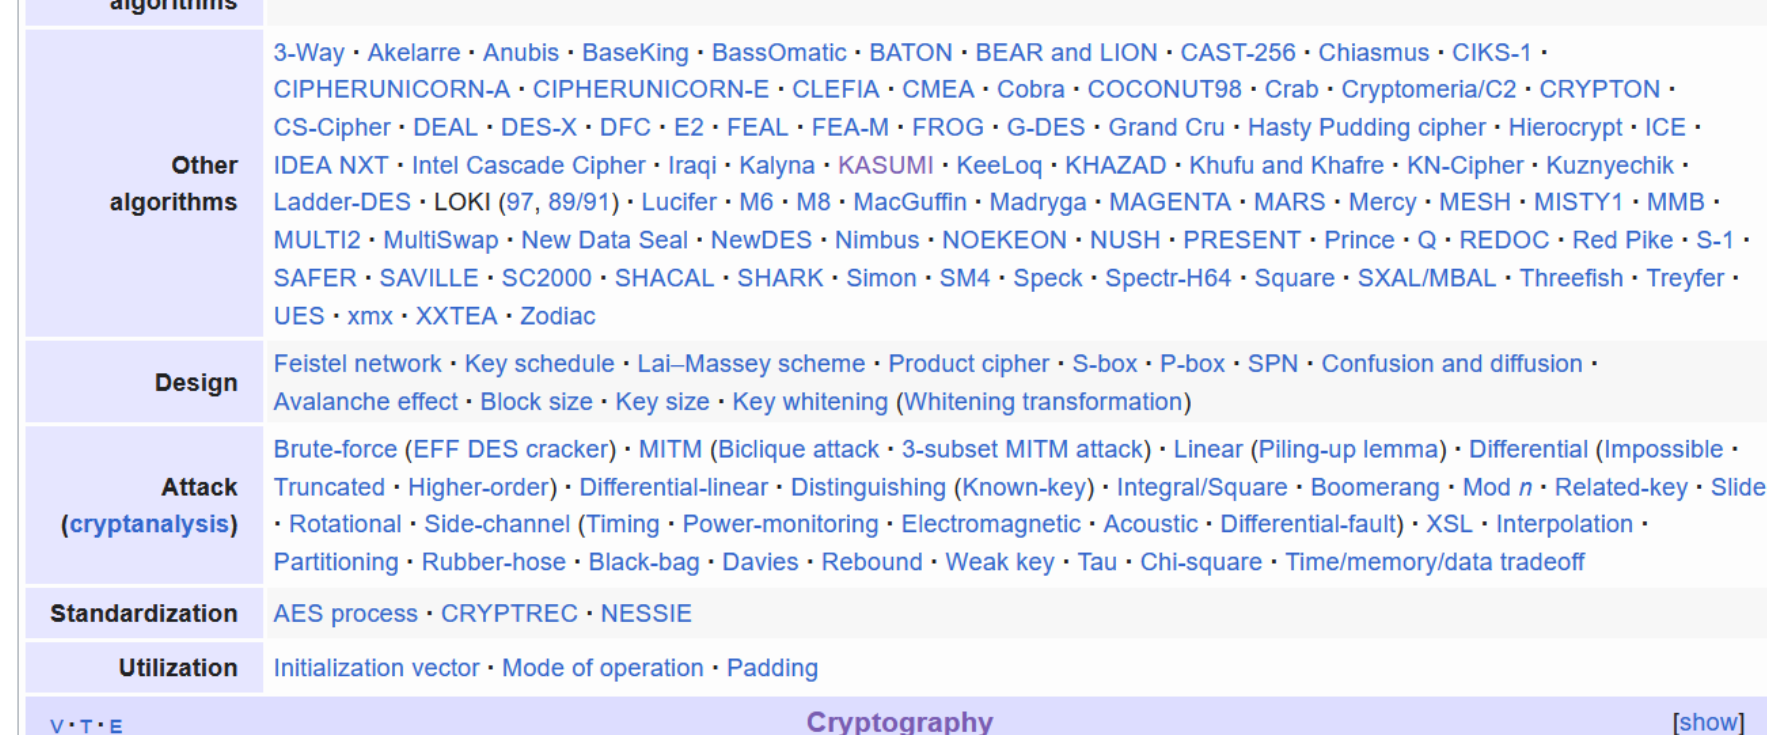
\includegraphics[width=193.20mm,height=201.96mm]{images/llm/page_008_img_01.png}%
\end{textblock*}

\newpage

% --- unit llm 9 ---
% === Halaman 9 (llm) ===

\section*{Mode Operasi \textit{Cipher} Blok}

\vspace{130.68mm}

\begin{itemize}
    \item Mode operasi: berkaitan dengan cara blok pesan dioperasikan sebelum dienkripsi/dekripsi oleh fungsi E dan D.
    \item Ada 5 mode operasi \textit{cipher} blok:
    \begin{enumerate}
        \item \textit{Electronic Code Book} (ECB)
        \item \textit{Cipher Block Chaining} (CBC)
        \item \textit{Cipher Feedback} (CFB)
        \item \textit{Output Feedback} (OFB)
        \item \textit{Counter Mode}
    \end{enumerate}
\end{itemize}

\vspace{10mm}

% deskripsi: Diagram blok proses enkripsi dan dekripsi menggunakan fungsi E dan D dengan kunci K, menunjukkan transformasi dari blok plaintext P menjadi blok ciphertexts C dan sebaliknya.
% bbox normalisasi: [0.5200, 0.4000, 0.9600, 0.8400]
\begin{textblock*}{92.40mm}(109.20mm,118.80mm)
\noindent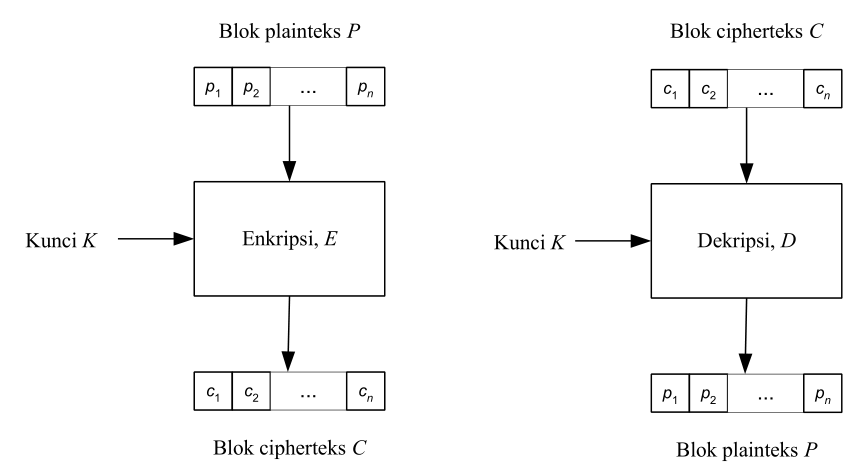
\includegraphics[width=92.40mm,height=130.68mm]{images/llm/page_009_img_01.png}%
\end{textblock*}

\newpage

% --- unit llm 10 ---
% === Halaman 10 (llm) ===

% (tidak ada teks dari model)

% deskripsi: Diagram hierarki yang menunjukkan berbagai Mode Operasi (Modes of operation) enkripsi blok, termasuk Electronic codebook (ECB), Cipher block chaining (CBC), Cipher feedback (CFB), Output feedback (OFB), dan Counter (CTR).
% bbox normalisasi: [0.7700, 0.3450, 0.9200, 0.6650]
\begin{textblock*}{31.50mm}(161.70mm,102.46mm)
\noindent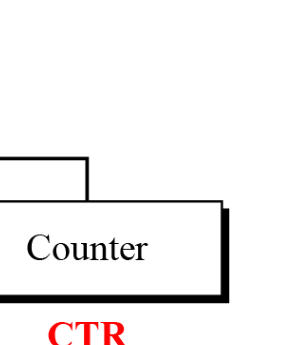
\includegraphics[width=31.50mm,height=95.04mm]{images/llm/page_010_img_01.png}%
\end{textblock*}

\newpage

% --- unit llm 11 ---
% === Halaman 11 (llm) ===

\section*{1. Electronic Code Book (ECB)}

\begin{itemize}
    \item Setiap blok plainteks $P_i$ dienkripsi secara individual dan independen dari blok lainnya menjadi blok cipherteks $C_i$.
    \item Enkripsi: \[ C_i = E_K(P_i) \]
    Dekripsi: \[ P_i = D_K(C_i) \]
\end{itemize}

yang dalam hal ini, $P_i$ dan $C_i$ masing-masing blok plainteks dan cipherteks ke-$i$.

\newpage

% --- unit llm 12 ---
% === Halaman 12 (llm) ===

\begin{center}
\textbf{Mode ECB}
\end{center}

\vspace{139.59mm}

E: Encryption \hfill D: Decryption \\
P$_i$: Plaintext block $i$ \hfill C$_i$: Ciphertext block $i$ \\
K: Secret key

\vspace{10mm}

% deskripsi: Diagram proses enkripsi dan dekripsi menggunakan mode Electronic Codebook (ECB), yang menunjukkan pengolahan blok plaintext menjadi ciphertext dan sebaliknya menggunakan kunci rahasia K.
% bbox normalisasi: [0.0000, 0.3800, 0.9600, 0.8500]
\begin{textblock*}{201.60mm}(0.00mm,112.86mm)
\noindent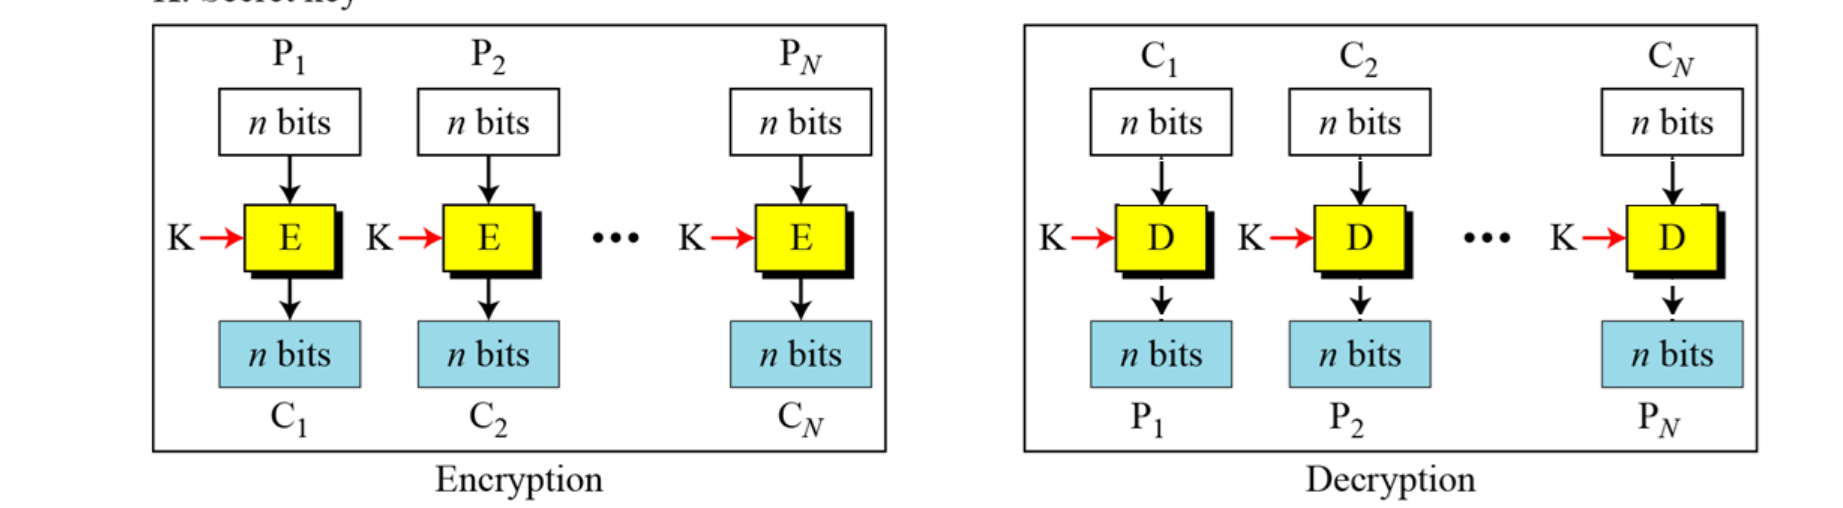
\includegraphics[width=201.60mm,height=139.59mm]{images/llm/page_012_img_01.png}%
\end{textblock*}

\newpage

% --- unit llm 13 ---
% === Halaman 13 (llm) ===

\begin{itemize}
  \item Contoh:
  \begin{itemize}
    \item Plainteks: \texttt{10100010001110101001}
    \item Bagi plainteks menjadi blok-blok 4-bit:
    \texttt{1010 0010 0011 1010 1001}
    ( dalam notasi HEX :A23A9)
  \end{itemize}
  \item Kunci (juga 4-bit): \texttt{1011}
  \item Misalkan fungsi enkripsi $E$ yang sederhana algoritmanya sbb:
  \begin{enumerate}
    \item XOR-kan blok plainteks $P_i$ dengan $K$
    \item geser secara \textit{wrapping} bit-bit dari hasil langkah 1 satu posisi ke kiri
  \end{enumerate}
\end{itemize}

\[ E_K(P) = (P \oplus K) \ll 1 \]

\newpage

% --- unit llm 14 ---
% === Halaman 14 (llm) ===

\textbf{Enkripsi:}

\[ E_K(P) = (P \oplus K) \ll 1 \]

\vspace{20mm}

Jadi, hasil enkripsi plainteks

\[ 10100010001110101001 \quad (\text{A23A9 dalam notasi HEX}) \]

adalah

\[ 00100011000100100100 \quad (\text{23124 dalam notasi HEX}) \]

% deskripsi: Proses perhitungan XOR antara dua deret biner, pergeseran 1 bit ke kiri, dan konversinya ke notasi hexadecimal.
% bbox normalisasi: [0.3200, 0.2300, 0.7300, 0.5200]
\begin{textblock*}{86.10mm}(67.20mm,68.31mm)
\noindent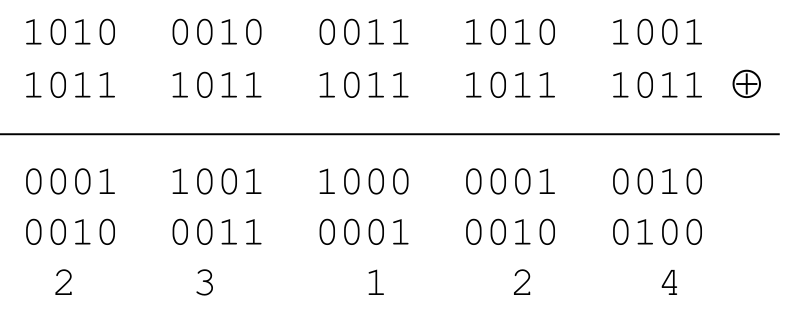
\includegraphics[width=86.10mm,height=86.13mm]{images/llm/page_014_img_01.png}%
\end{textblock*}

\newpage

% --- unit llm 15 ---
% === Halaman 15 (llm) ===

\begin{itemize}
  \item Pada mode ECB, blok plainteks yang sama selalu dienkripsi menjadi blok cipherteks yang sama.
\end{itemize}

\vspace{10mm}

\begin{itemize}
  \item Pada contoh di atas, blok 1010 muncul dua kali dan selalu dienkripsi menjadi 0010.
\end{itemize}

% deskripsi: Ilustrasi proses enkripsi mode ECB yang menunjukkan operasi XOR antara plainteks dan kunci, pergeseran bit, dan konversi ke notasi HEX, dengan penekanan pada blok 1010 yang menghasilkan output 0010 secara konsisten.
% bbox normalisasi: [0.1600, 0.2900, 0.7600, 0.6100]
\begin{textblock*}{126.00mm}(33.60mm,86.13mm)
\noindent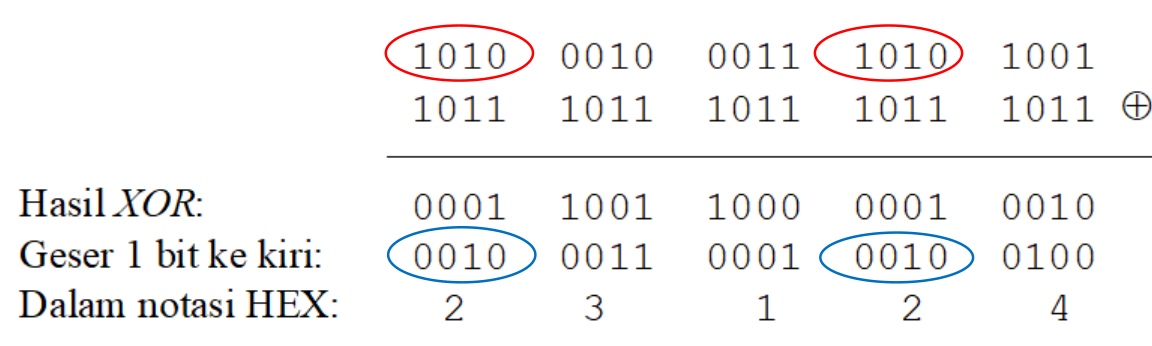
\includegraphics[width=126.00mm,height=95.04mm]{images/llm/page_015_img_01.png}%
\end{textblock*}

\newpage

% --- unit llm 16 ---
% === Halaman 16 (llm) ===

\vspace{112.86mm}

\begin{itemize}
  \item Karena setiap blok plainteks yang sama selalu dienkripsi menjadi blok cipherteks yang sama, maka secara teoritis dimungkinkan membuat buku kode plainteks dan cipherteks yang berkoresponden (asal kata \textit{``code book''} di dalam ECB ). Enkripsi/dekripsi dilakukan dengan \textit{look up table}.
  \vspace{20mm}
  \item Untuk setiap kunci K yang berbeda, dibuat buku kode yang berbeda pula. Jika panjang kunci n bit, maka terdapat $2^n$ buku kode.
\end{itemize}

% deskripsi: Tabel contoh buku kode (look up table) yang memetakan nilai Plainteks ke Cipherteks dalam format biner.
% bbox normalisasi: [0.1300, 0.2900, 0.4300, 0.6700]
\begin{textblock*}{63.00mm}(27.30mm,86.13mm)
\noindent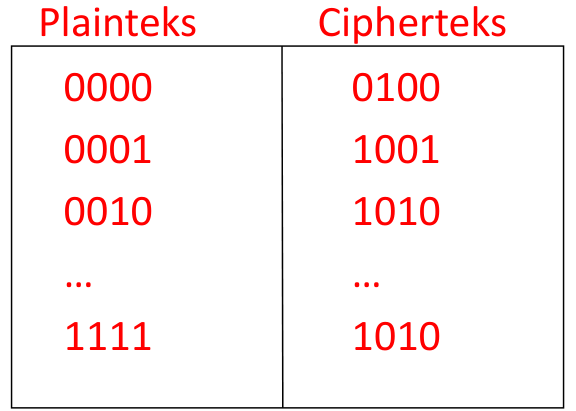
\includegraphics[width=63.00mm,height=112.86mm]{images/llm/page_016_img_01.png}%
\end{textblock*}

\newpage

% --- unit llm 17 ---
% === Halaman 17 (llm) ===

\begin{itemize}
    \item Jumlah entri (baris) di dalam setiap buku kode untuk adalah $2^n$.
    \item Namun, semakin besar ukuran blok, semakin besar pula ukuran buku kodenya.
    \item Misalkan jika blok berukuran 64 bit, maka buku kode terdiri dari $2^{64}$ buah kode (\textit{entry}), yang berarti terlalu besar untuk disimpan. Lagipula, setiap kunci mempunyai buku kode yang berbeda.
\end{itemize}

\newpage

% --- unit llm 18 ---
% === Halaman 18 (llm) ===

\begin{itemize}
    \item Jika panjang plainteks tidak habis dibagi dengan ukuran blok, maka blok terakhir berukuran lebih pendek daripada blok-blok lainnya.
    \item Untuk itu, kita tambahkan bit-bit \textit{padding} untuk menutupi kekurangan bit blok.
    \item Bit-bit padding misalnya bit 0 semua, atau bit 1 semua, atau bit 0 dan bit 1 berselang-seling.
    \item Contoh: Ukuran blok 8 bit: \textcolor{red}{10001101} \textcolor{red}{00101001} \textcolor{red}{10110}\textcolor{blue}{000}\\
    Blok terakhir hanya 5 bit, ditambah 3 bit \textit{padding} (\textcolor{blue}{warna biru})
\end{itemize}

\newpage

% --- unit llm 19 ---
% === Halaman 19 (llm) ===

\section*{Kelebihan Mode $ECB$}

\begin{enumerate}
    \item Karena tiap blok plainteks dienkripsi secara independen, maka kita tidak perlu mengenkripsi pesan secara sekuensial/linier.
\end{enumerate}

\begin{itemize}
    \item Kita dapat mengenkripsi 5 blok pertama, kemudian blok-blok di akhir, dan kembali ke blok-blok di tengah dan seterusnya.
    \item Mode $ECB$ cocok untuk mengenkripsi isi arsip (\textit{file}) yang diakses secara acak, misalnya arsip-arsip basisdata.
    \item Jika basisdata dienkripsi dengan mode $ECB$, maka sembarang \textit{record} dapat dienkripsi secara independen dari \textit{record} lainnya (dengan asumsi setiap \textit{record} terdiri dari sejumlah blok diskrit yang sama banyaknya).
\end{itemize}

\newpage

% --- unit llm 20 ---
% === Halaman 20 (llm) ===

\begin{enumerate}
  \item[2.] Kesalahan 1 atau lebih bit pada blok cipherteks hanya mempengaruhi cipherteks yang bersangkutan pada proses dekripsi.
\end{enumerate}

Blok-blok cipherteks lainnya bila didekripsi tidak terpengaruh oleh kesalahan bit cipherteks tersebut.

\newpage

% --- unit llm 21 ---
% === Halaman 21 (llm) ===

\section*{Kelemahan Mode ECB}

\begin{enumerate}
    \item Karena plainteks sering mengandung bagian yang berulang (sehingga terdapat blok-blok plainteks yang sama), maka enkripsinya menghasilkan blok cipherteks yang sama pula
    \begin{itemize}
        \item contoh berulang: spasi panjang
        \item mudah diserang secara statisitik dengan analisis frekuensi
    \end{itemize}
\end{enumerate}

\newpage

% --- unit llm 22 ---
% === Halaman 22 (llm) ===

2. Pihak lawan dapat memanipulasi cipherteks untuk ``membodohi'' atau mengelabui penerima pesan.

Contoh: Seseorang mengirim pesan

``Uang ditransfer lima satu juta rupiah''

\newpage

% --- unit llm 23 ---
% === Halaman 23 (llm) ===

Andaikan kriptanalis mengetahui ukuran blok = 2 karakter (16 bit), spasi diabaikan.

Blok-blok cipherteks:
\[ C_{1}, C_{2}, C_{3}, C_{4}, C_{5}, C_{6}, C_{7}, \color{red}{C_{8}, C_{9}}, C_{10}, C_{11}, C_{12}, C_{13}, C_{14}, C_{15}, C_{16} \]

Misalkan kriptanalis mengethaui posisi pesan yang berkaitan dengan nominal uang, yaitu blok $C_{8}$ dan $C_{9}$.

Kriptanalis membuang blok cipherteks $C_{8}$ dan $C_{9}$ :
\[ C_{1}, C_{2}, C_{3}, C_{4}, C_{5}, C_{6}, C_{7}, C_{10}, C_{11}, C_{12}, C_{13}, C_{14}, C_{15}, C_{16} \]

\newpage

% --- unit llm 24 ---
% === Halaman 24 (llm) ===

Penerima pesan mendekripsi cipherteks yang sudah dimanipulasi dengan kunci yang benar menjadi

\vspace{10mm}

Karena dekripsi menghasilkan pesan yang bermakna, maka penerima menyimpulkan bahwa uang yang dikirim kepadanya sebesar satu juta rupiah.

% deskripsi: Teks berwarna merah yang menunjukkan hasil dekripsi pesan: 'Uang ditransfer satu juta rupiah'
% bbox normalisasi: [0.1940, 0.3750, 0.7580, 0.4250]
\begin{textblock*}{118.44mm}(40.74mm,111.38mm)
\noindent
\includegraphics[width=118.44mm,height=14.85mm]{images/llm/page_024_img_01.png}%
\end{textblock*}

\newpage

% --- unit llm 25 ---
% === Halaman 25 (llm) ===

\begin{itemize}
    \item Cara mengatasi kelemahan ini: enkripsi tiap blok individual bergantung pada semua blok-blok sebelumnya.
    \item Prinsip ini mendasari mode \textit{Cipher Block Chaining} (CBC).
\end{itemize}

\newpage

% --- unit llm 26 ---
% === Halaman 26 (llm) ===

\section*{Cipher Block Chaining(CBC)}

\begin{itemize}
    \item Tujuan: membuat ketergantungan antar blok (mengatasi kelemahan mode ECB).
    \item Setiap blok cipherteks bergantung tidak hanya pada blok plainteksnya tetapi juga pada seluruh blok plainteks sebelumnya.
    \item Hasil enkripsi blok sebelumnya di-umpan-balikkan ke dalam enkripsi blok yang current.
    \item Enkripsi blok pertama memerlukan blok semu ($C_0$) yang disebut IV (initialization vector).
    \item IV dapat diberikan oleh pengguna atau dibangkitkan secara acak oleh program.
    \item Pada dekripsi, blok plainteks diperoleh dengan cara meng-XOR-kan IV dengan hasil dekripsi terhadap blok cipherteks pertama.
\end{itemize}

\newpage

% --- unit llm 27 ---
% === Halaman 27 (llm) ===

\vspace{135.73mm}

(a) Skema enkripsi mode CBC

\begin{itemize}
    \item[Encryption:]
    \[ C_0 = \text{IV} \]
    \[ C_i = E_K (P_i \oplus C_{i-1}) \]
\end{itemize}

\vspace{30mm}

(b) Skema dekripsi mode CBC

\begin{itemize}
    \item[Decryption:]
    \[ C_0 = \text{IV} \]
    \[ P_i = D_K (C_i) \oplus C_{i-1} \]
\end{itemize}

% deskripsi: Diagram alur proses enkripsi Cipher Block Chaining (CBC) yang menunjukkan penggunaan Initialization Vector (IV), operasi XOR antara plaintext dan ciphertext sebelumnya, serta blok enkripsi E dengan kunci K.
% bbox normalisasi: [0.3020, 0.0250, 0.9450, 0.4820]
\begin{textblock*}{135.03mm}(63.42mm,7.43mm)
\noindent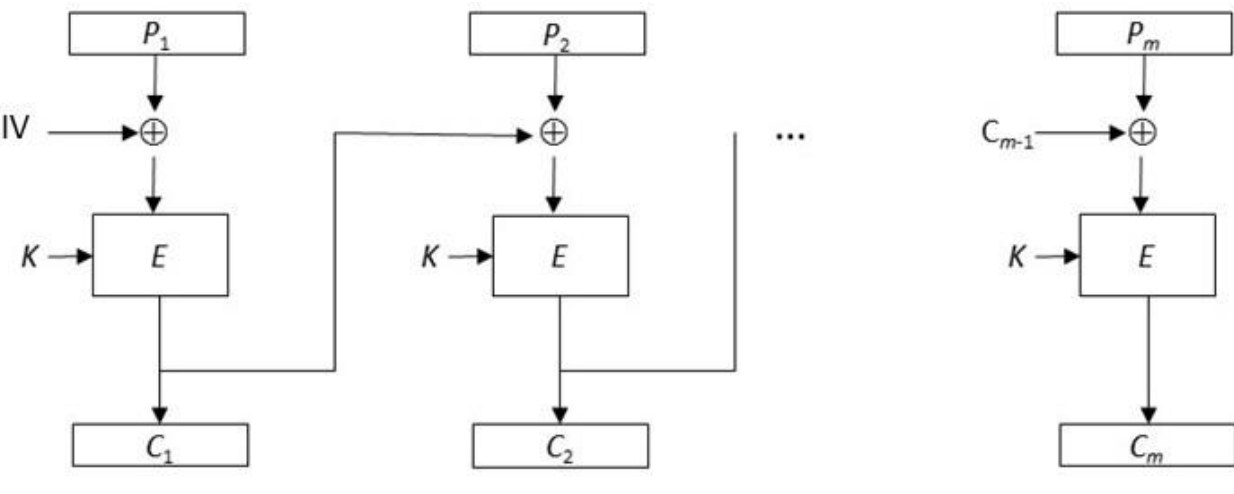
\includegraphics[width=135.03mm,height=135.73mm]{images/llm/page_027_img_01.png}%
\end{textblock*}

% deskripsi: Diagram alur proses dekripsi Cipher Block Chaining (CBC) yang menunjukkan penggunaan blok dekripsi D dengan kunci K, dan operasi XOR antara hasil dekripsi dengan ciphertext sebelumnya untuk mendapatkan plaintext.
% bbox normalisasi: [0.3020, 0.5350, 0.9450, 0.9700]
\begin{textblock*}{135.03mm}(63.42mm,158.90mm)
\noindent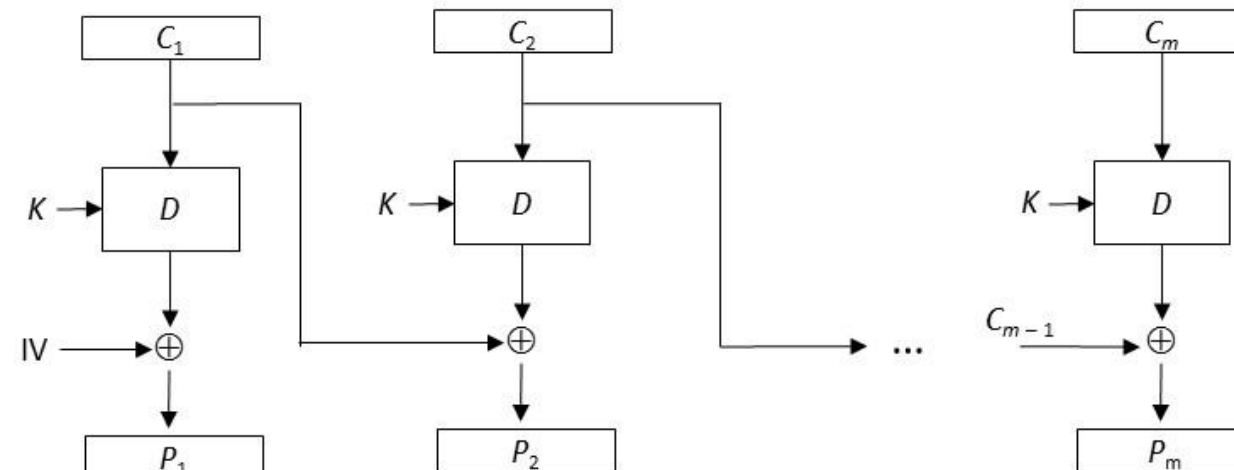
\includegraphics[width=135.03mm,height=129.19mm]{images/llm/page_027_img_02.png}%
\end{textblock*}

\newpage

% --- unit llm 28 ---
% === Halaman 28 (llm) ===

\begin{center}
\Large Mode CBC
\end{center}

\vspace{60mm}

\begin{tabular}{|c|c|c|}
\hline
CBC & $\begin{aligned} C_1 &= E(K, [P_1 \oplus IV]) \\ C_j &= E(K, [P_j \oplus C_{j-1}]) \ j = 2, \dots, N \end{aligned}$ & $\begin{aligned} P_1 &= D(K, C_1) \oplus IV \\ P_j &= D(K, C_j) \oplus C_{j-1} \ j = 2, \dots, N \end{aligned}$ \\
\hline
\end{tabular}

% deskripsi: Diagram proses enkripsi dan dekripsi menggunakan mode Cipher Block Chaining (CBC). Bagian (a) menunjukkan proses enkripsi di mana plaintext di-XOR dengan IV atau ciphertext sebelumnya sebelum dienkripsi. Bagian (b) menunjukkan proses dekripsi di mana ciphertext didekripsi terlebih dahulu lalu di-XOR dengan IV atau ciphertext sebelumnya untuk mendapatkan plaintext.
% bbox normalisasi: [0.0180, 0.2800, 0.9820, 0.6300]
\begin{textblock*}{202.44mm}(3.78mm,83.16mm)
\noindent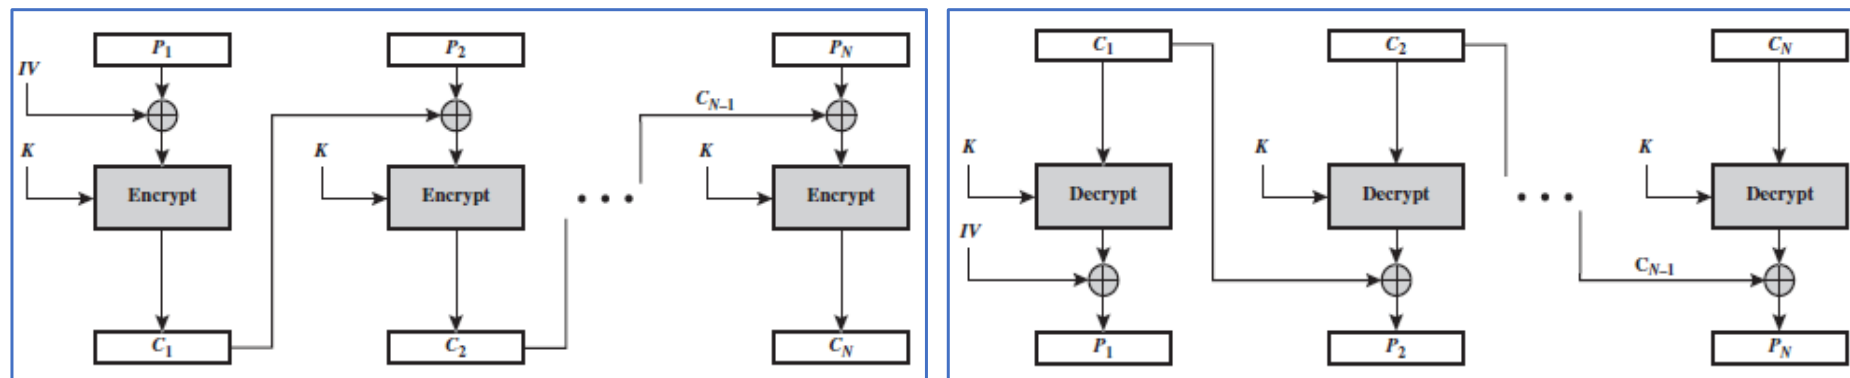
\includegraphics[width=202.44mm,height=103.95mm]{images/llm/page_028_img_01.png}%
\end{textblock*}

\newpage

% --- unit llm 29 ---
% === Halaman 29 (llm) ===

\textbf{Contoh 9.8.} Tinjau kembali plainteks dari Contoh 9.6:

\begin{center}
$10100010001110101001$
\end{center}

Bagi plainteks menjadi blok-blok yang berukuran 4 bit:

\begin{center}
$1010 \quad 0010 \quad 0011 \quad 1010 \quad 1001$
\end{center}

atau dalam notasi HEX adalah $\text{A23A9}$.

Misalkan kunci ($K$) yang digunakan adalah (panjangnya juga 4 bit)

\begin{center}
$1011$
\end{center}

atau dalam notasi HEX adalah $\text{B}$. Sedangkan $IV$ yang digunakan seluruhnya bit 0 (Jadi, $C_0 = 0000$)

Fungsi enkripsi $E$ yang digunakan sama seperti sebelumnya: XOR-kan blok plainteks $P_i$ dengan $K$, kemudian geser secara \textit{wrapping} bit-bit dari $P_i \oplus K$ satu posisi ke kiri.

\[ E_K(P) = (P \oplus K) \ll 1 \]

\newpage

% --- unit llm 30 ---
% === Halaman 30 (llm) ===

\vspace{98.01mm}

$C_1$ diperoleh sebagai berikut:
\[ P_1 \oplus C_0 = 1010 \oplus 0000 = 1010 \]

% deskripsi: Diagram blok proses enkripsi cipher feedback mode (CFB) yang menunjukkan aliran data melalui fungsi E dan operasi XOR dengan plaintext P untuk menghasilkan ciphertext C.
% bbox normalisasi: [0.5200, 0.3500, 0.9700, 0.6800]
\begin{textblock*}{94.50mm}(109.20mm,103.95mm)
\noindent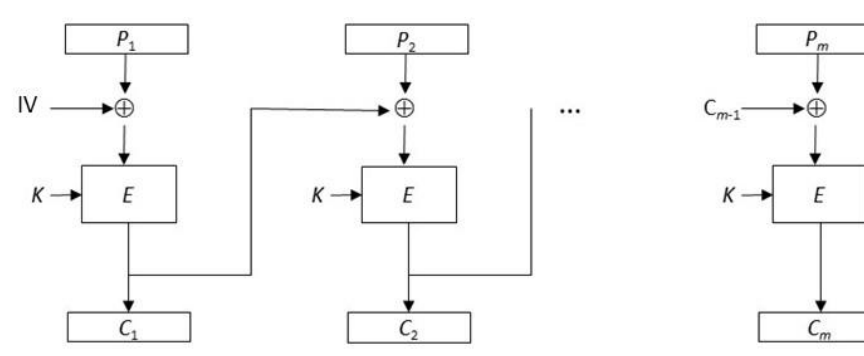
\includegraphics[width=94.50mm,height=98.01mm]{images/llm/page_030_img_01.png}%
\end{textblock*}

\newpage

% --- unit llm 31 ---
% === Halaman 31 (llm) ===

Demikian seterusnya, sehingga plainteks dan cipherteks hasilnya adalah:
\begin{align*}
\text{Pesan (plainteks):} & \quad A23A9 \\
\text{Cipherteks (mode $ECB$):} & \quad 23124 \\
\text{Cipherteks (mode $CBC$):} & \quad 27FBF
\end{align*}

\newpage

% --- unit llm 32 ---
% === Halaman 32 (llm) ===

\section*{Kelebihan Mode CBC}

Blok-blok plainteks yang sama tidak selalu menghasilkan blok-blok cipherteks yang sama

Oleh karena blok-blok plainteks yang sama tidak menghasilkan blok-blok cipherteks yang sama, maka kriptanalisis menjadi lebih sulit.

Inilah alasan utama penggunaan mode CBC.

\newpage

% --- unit llm 33 ---
% === Halaman 33 (llm) ===

\vspace{106.92mm}

\section*{Kelemahan Mode CBC}

\vspace{106.92mm}

\begin{enumerate}
    \item Kesalahan satu bit pada sebuah blok plainteks akan menghasilkan kesalahan pada blok cipherteks yang berkoresponden dan kesalahan tersebut merambat ke semua blok cipherteks berikutnya.
    \vspace{50mm}
    \item Tetapi, hal ini berkebalikan pada proses dekripsi. Kesalahan satu bit pada blok cipherteks hanya mempengaruhi blok plainteks yang berkoresponden dan satu bit pada blok plainteks berikutnya (pada posisi bit yang berkoresponden pula).
\end{enumerate}

% deskripsi: Diagram proses enkripsi pada mode CBC (Cipher Block Chaining) yang menunjukkan aliran data dari plainteks P ke cipherteks C menggunakan kunci K dan Initialization Vector (IV).
% bbox normalisasi: [0.5300, 0.1200, 0.9800, 0.4800]
\begin{textblock*}{94.50mm}(111.30mm,35.64mm)
\noindent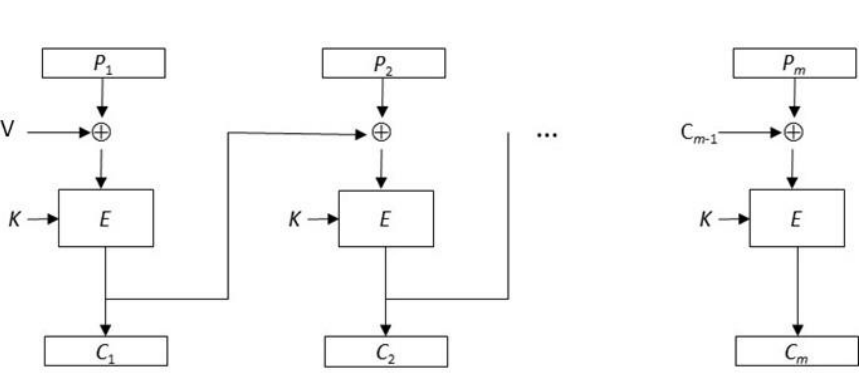
\includegraphics[width=94.50mm,height=106.92mm]{images/llm/page_033_img_01.png}%
\end{textblock*}

% deskripsi: Diagram proses dekripsi pada mode CBC (Cipher Block Chaining) yang menunjukkan aliran data dari cipherteks C kembali menjadi plainteks P menggunakan kunci K dan Initialization Vector (IV).
% bbox normalisasi: [0.5300, 0.5300, 0.9800, 0.8900]
\begin{textblock*}{94.50mm}(111.30mm,157.41mm)
\noindent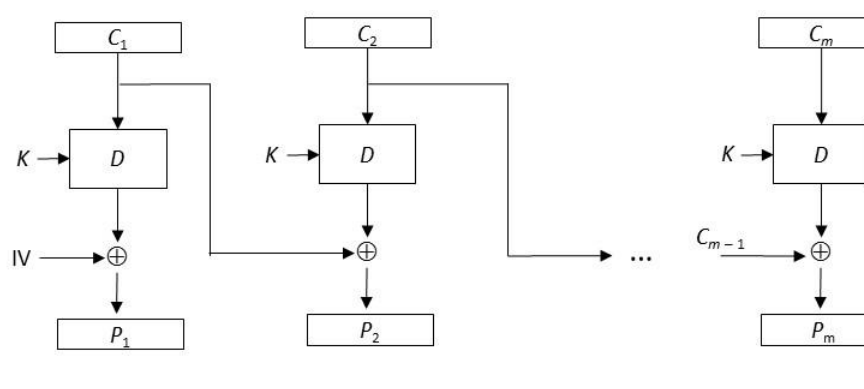
\includegraphics[width=94.50mm,height=106.92mm]{images/llm/page_033_img_02.png}%
\end{textblock*}

\newpage

% --- unit llm 34 ---
% === Halaman 34 (llm) ===

\section*{Cipher-Feedback (CFB)}

\begin{itemize}
    \item Mengatasi kekurangan pada mode $CBC$ apabila diterapkan pada pengiriman data yang belum mencapai ukuran satu blok
    \item Data dienkripsi dalam unit yang lebih kecil $(s)$ daripada ukuran blok $(b)$.
    \item Unit data yang dienkripsi panjangnya bisa 1 bit, 2 bit, 4-bit, 8 bit, dan lain-lain.
    \item Bila unit yang dienkripsi adalah satu karakter setiap kalinya, maka mode $CFB$-nya disebut $CFB$ 8-bit.
\end{itemize}

\newpage

% --- unit llm 35 ---
% === Halaman 35 (llm) ===

\begin{itemize}
    \item $CFB$ $s$-bit mengenkripsi plainteks berukuran $s$ bit setiap kalinya, $s \le b$ ($b =$ ukuran blok dalam satuan bit).
    \item Dengan kata lain, $CFB$ $s$-bit memperlakukan $cipher$ blok sama seperti pada $cipher$ alir.
    \item Mode $CFB$ membutuhkan sebuah antrian (\textit{shift register}) yang berukuran sama dengan ukuran blok masukan ($b$ bit).
    \item Tinjau mode $CFB$ 8-bit yang bekerja pada blok berukuran 64-bit pada gambar berikut ($s = 8, b = 64$):
\end{itemize}

\newpage

% --- unit llm 36 ---
% === Halaman 36 (llm) ===

\textcolor{red}{\huge Mode CFB-8 bit untuk ukuran blok 64 bit (= 8 byte)}

\vspace{10mm}

(a) Enkripsi

\vspace{10mm}

(b) Dekripsi

% deskripsi: Diagram proses enkripsi Mode CFB-8 bit yang menunjukkan shift register 8-byte, blok enkripsi E dengan kunci K, operasi XOR antara plaintext p_i dan keystream k_i untuk menghasilkan ciphertext c_i.
% bbox normalisasi: [0.1700, 0.2000, 0.4200, 0.8200]
\begin{textblock*}{52.50mm}(35.70mm,59.40mm)
\noindent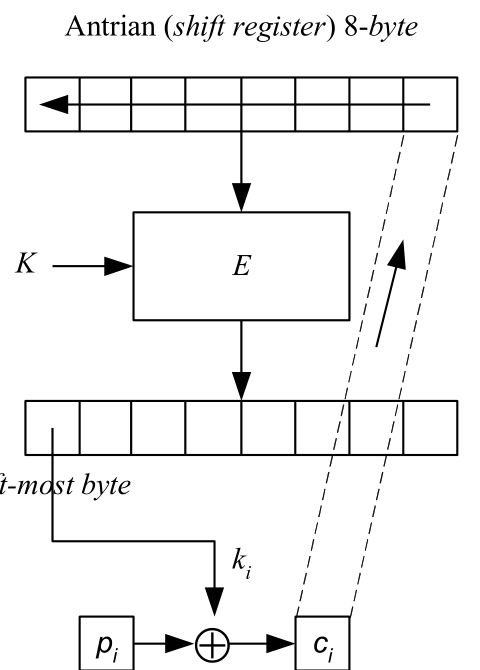
\includegraphics[width=52.50mm,height=184.14mm]{images/llm/page_036_img_01.png}%
\end{textblock*}

% deskripsi: Diagram proses dekripsi Mode CFB-8 bit yang menunjukkan shift register 8-byte, blok enkripsi E dengan kunci K, operasi XOR antara ciphertext c_i dan keystream k_i untuk mengembalikan plaintext p_i.
% bbox normalisasi: [0.5600, 0.2000, 0.8400, 0.8200]
\begin{textblock*}{58.80mm}(117.60mm,59.40mm)
\noindent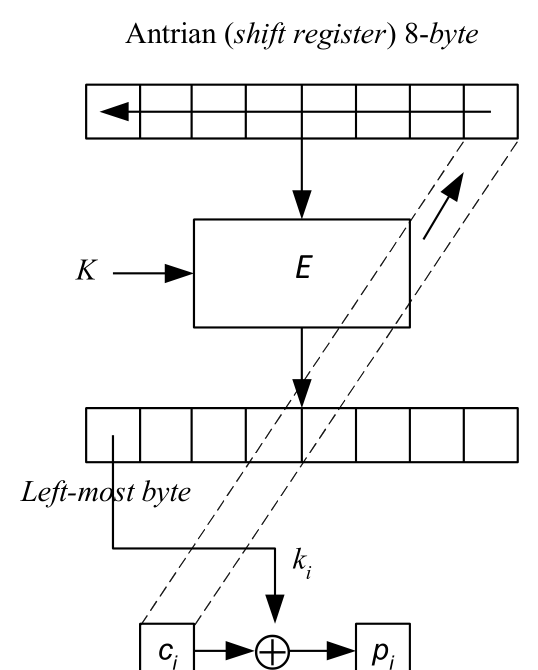
\includegraphics[width=58.80mm,height=184.14mm]{images/llm/page_036_img_02.png}%
\end{textblock*}

\newpage

% --- unit llm 37 ---
% === Halaman 37 (llm) ===

Secara matematis, mode $CFB$ $s$-bit dapat dinyatakan sebagai:

\begin{align*}
\text{Enkripsi:}\\ C_j &= P_j \oplus \text{MSB}_s(E_K(X_j)) \\
X_{j+1} &= \text{LSB}_{b-s}(X_j) \parallel C_i
\end{align*}
\begin{align*}
\text{Dekripsi:}\\ P_j &= C_i \oplus \text{MSB}_s(E_K(X_j)) \\
X_{j+1} &= \text{LSB}_{b-s}(X_j) \parallel C_i
\end{align*}

yang dalam hal ini,
\begin{itemize}
    \item $j = 1, 2, 3, ..., m$
    \item $X_j = \text{antrian bergeser, dengan } X_1 = IV$
    \item $E = \text{fungsi enkripsi}$
    \item $K = \text{kunci}$
    \item $b = \text{panjang blok enkripsi}$
    \item $s = \text{panjang unit enkripsi}$
    \item $\parallel = \text{operator penyambungan (concatenation)}$
    \item $\text{MSB} = \text{Most Significant Byte}$
\end{itemize}

\newpage

% --- unit llm 38 ---
% === Halaman 38 (llm) ===

\section*{Mode CFB}

\vspace{60mm}

\textbf{Enkripsi:}
\[ C_j = P_j \oplus MSB_s(E_K(X_j)) \]
\[ X_{j+1} = LSB_{b-s}(X_j) \parallel C_i \]

\textbf{Dekripsi:}
\[ P_j = C_i \oplus MSB_s(E_K(X_j)) \]
\[ X_{j+1} = LSB_{b-s}(X_j) \parallel C_i \]

\vspace{10mm}

Mode CFB mengoperasikan \textbf{block cipher seperti stream cipher!!}

% deskripsi: Diagram blok proses enkripsi Mode CFB yang menunjukkan penggunaan IV, register geser, operasi enkripsi, dan XOR dengan plaintext untuk menghasilkan ciphertext.
% bbox normalisasi: [0.0120, 0.1270, 0.4970, 0.6370]
\begin{textblock*}{101.85mm}(2.52mm,37.72mm)
\noindent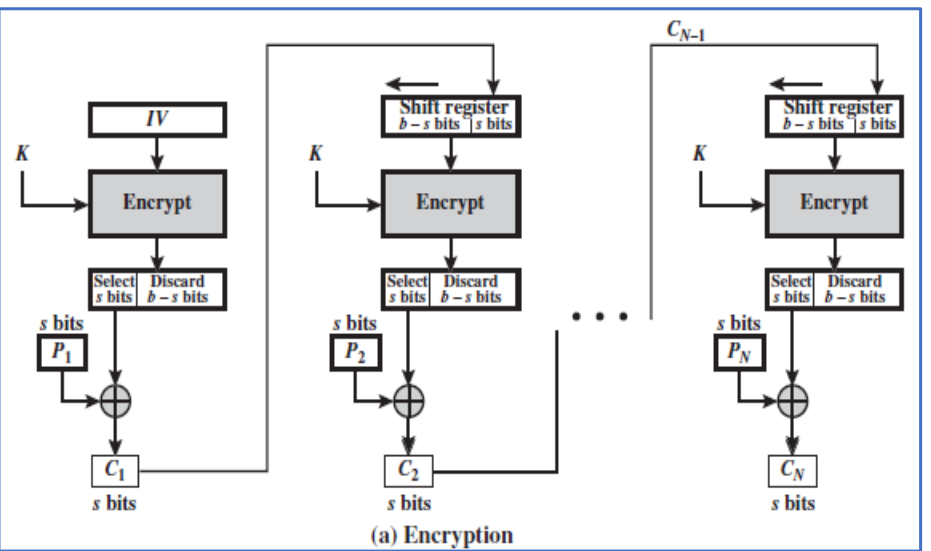
\includegraphics[width=101.85mm,height=151.47mm]{images/llm/page_038_img_01.png}%
\end{textblock*}

% deskripsi: Diagram blok proses dekripsi Mode CFB yang menunjukkan proses pemulihan plaintext menggunakan ciphertext dan output dari cipher block yang terenkripsi.
% bbox normalisasi: [0.5030, 0.1270, 0.9880, 0.6370]
\begin{textblock*}{101.85mm}(105.63mm,37.72mm)
\noindent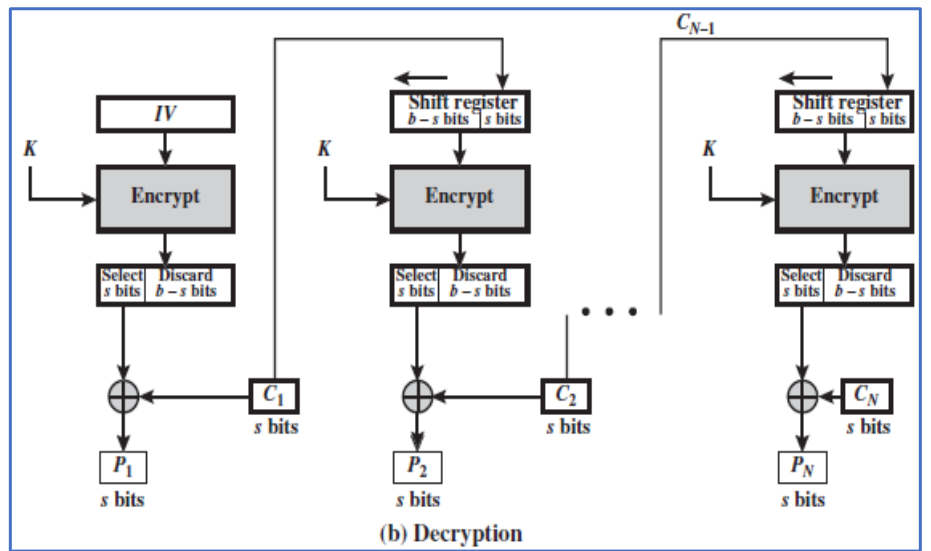
\includegraphics[width=101.85mm,height=151.47mm]{images/llm/page_038_img_02.png}%
\end{textblock*}

\newpage

% --- unit llm 39 ---
% === Halaman 39 (llm) ===

\begin{itemize}
  \item Jika $b = s$, maka mode $CFB$ $b$-bit adalah sbb:
\end{itemize}

\vspace{109.89mm}

\vspace{10mm}
(a) Enkripsi

\vspace{103.95mm}

\vspace{40mm}
(b) Dekripsi

% deskripsi: Diagram alur proses enkripsi menggunakan mode Cipher Feedback (CFB) dengan b = s, menunjukkan penggunaan IV, blok enkripsi Ek, plaintext P, dan ciphertext C.
% bbox normalisasi: [0.2600, 0.1300, 0.9400, 0.5000]
\begin{textblock*}{142.80mm}(54.60mm,38.61mm)
\noindent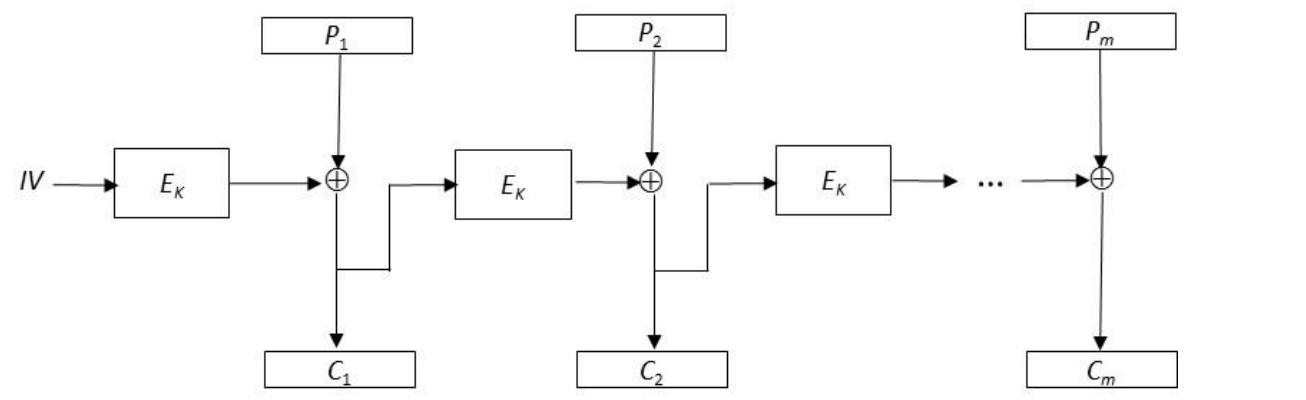
\includegraphics[width=142.80mm,height=109.89mm]{images/llm/page_039_img_01.png}%
\end{textblock*}

% deskripsi: Diagram alur proses dekripsi menggunakan mode Cipher Feedback (CFB) dengan b = s, menunjukkan bagaimana ciphertext C digunakan sebagai input untuk menghasilkan plaintext P.
% bbox normalisasi: [0.2600, 0.5800, 0.9400, 0.9300]
\begin{textblock*}{142.80mm}(54.60mm,172.26mm)
\noindent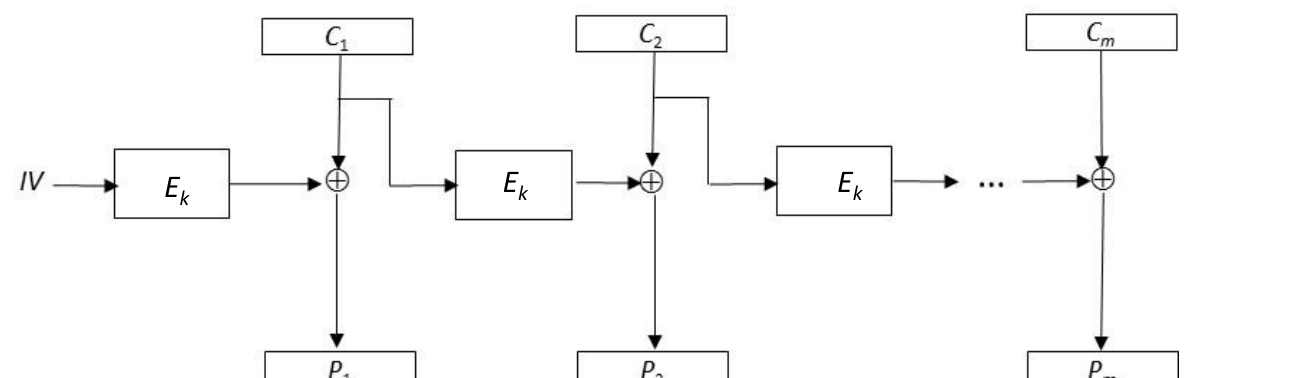
\includegraphics[width=142.80mm,height=103.95mm]{images/llm/page_039_img_02.png}%
\end{textblock*}

\newpage

% --- unit llm 40 ---
% === Halaman 40 (llm) ===

\begin{itemize}
  \item Dari Gambar tersebut dapat dilihat bahwa:

\vspace{115.83mm}

  \begin{align*}
    C_i &= P_i \oplus E_k(C_{i-1}) \\
    P_i &= C_i \oplus D_k(C_{i-1})
  \end{align*}

  yang dalam hal ini, $C_0 = IV$.

  \vspace{20mm}

  \item Kesalahan 1-bit pada suatu blok plainteks tertentu akan merambat pada blok cipherteks yang berkoresponden dan blok-blok cipherteks selanjutnya pada proses enkripsi.
\end{itemize}

% deskripsi: Diagram alir proses enkripsi Cipher Block Chaining (CBC) yang menunjukkan penggunaan IV, blok plainteks P, fungsi enkripsi Ek, dan hasil cipherteks C.
% bbox normalisasi: [0.4400, 0.1900, 0.9700, 0.5800]
\begin{textblock*}{111.30mm}(92.40mm,56.43mm)
\noindent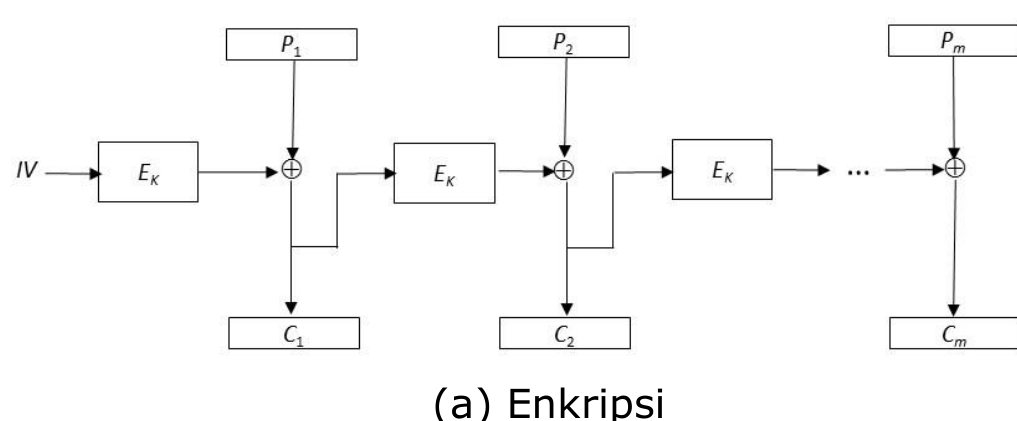
\includegraphics[width=111.30mm,height=115.83mm]{images/llm/page_040_img_01.png}%
\end{textblock*}

\newpage

% --- unit llm 41 ---
% === Halaman 41 (llm) ===

\vspace{20mm}

(b) Dekripsi

\vspace{10mm}

Hal yang kebalikan terjadi pada proses dekripsi. Kesalahan 1 bit pada suatu blok cipherteks tertentu hanya menghasilkan kesalahan dekripsi pada blok plainteks yang bersangkutan dan satu blok plainteks berikutnya.

% deskripsi: Diagram alur proses dekripsi blok cipher menggunakan mode operasi kriptografi, menunjukkan penggunaan Initialization Vector (IV), blok cipherteks (C), fungsi dekripsi (D_K), dan blok plainteks (P).
% bbox normalisasi: [0.1400, 0.1000, 0.7400, 0.4700]
\begin{textblock*}{126.00mm}(29.40mm,29.70mm)
\noindent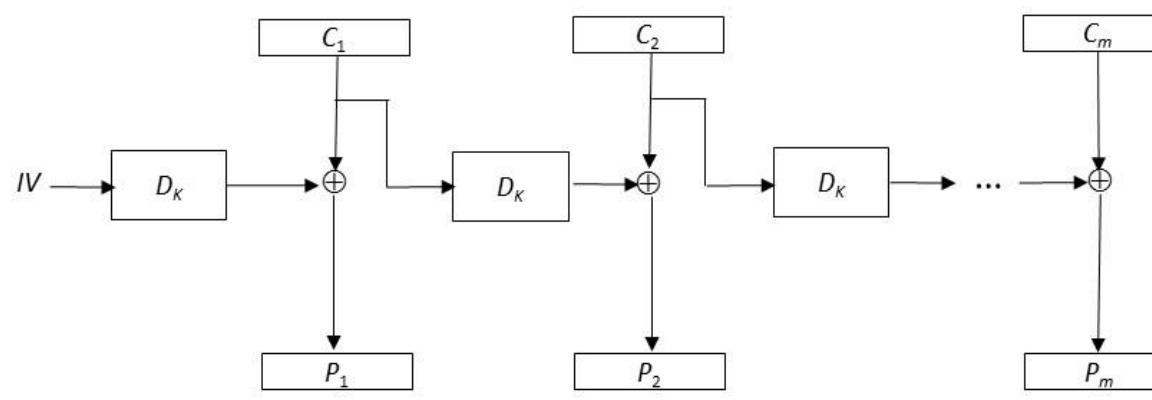
\includegraphics[width=126.00mm,height=109.89mm]{images/llm/page_041_img_01.png}%
\end{textblock*}

\newpage

% --- unit llm 42 ---
% === Halaman 42 (llm) ===

\section*{Output-Feedback (OFB)}

\vspace{187.11mm}

\begin{itemize}
    \item Mode $OFB$ mirip dengan mode $CFB$, kecuali $s$-bit dari hasil enkripsi antrian disalin menjadi elemen posisi paling kanan di antrian.
\end{itemize}

\vspace{60mm}

\begin{center}
    (a) Enkripsi \quad \quad \quad (b) Dekripsi
\end{center}

% deskripsi: Diagram blok proses enkripsi Output-Feedback (OFB) 8-bit yang menunjukkan aliran data melalui shift register, blok enkripsi E dengan kunci K, dan operasi XOR untuk menghasilkan ciphertext ci dari plaintext pi.
% bbox normalisasi: [0.1700, 0.3000, 0.4400, 0.9300]
\begin{textblock*}{56.70mm}(35.70mm,89.10mm)
\noindent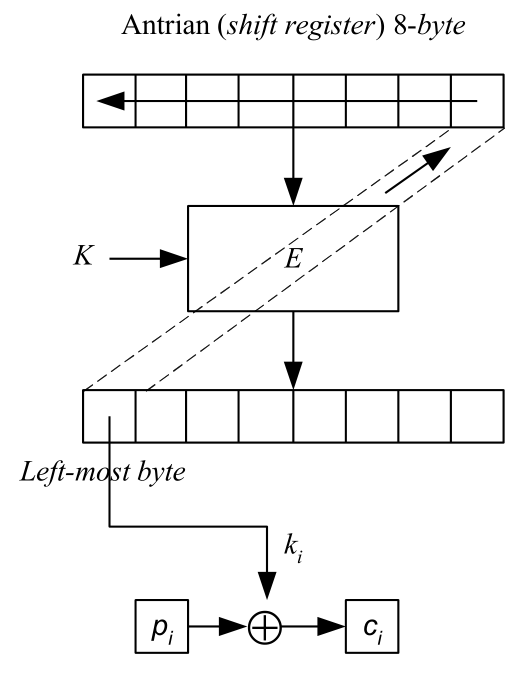
\includegraphics[width=56.70mm,height=187.11mm]{images/llm/page_042_img_01.png}%
\end{textblock*}

% deskripsi: Diagram blok proses dekripsi Output-Feedback (OFB) 8-bit yang menunjukkan proses yang identik dengan enkripsi, di mana ciphertext ci di-XOR dengan keystream ki untuk mendapatkan kembali plaintext pi.
% bbox normalisasi: [0.5800, 0.3000, 0.8500, 0.9300]
\begin{textblock*}{56.70mm}(121.80mm,89.10mm)
\noindent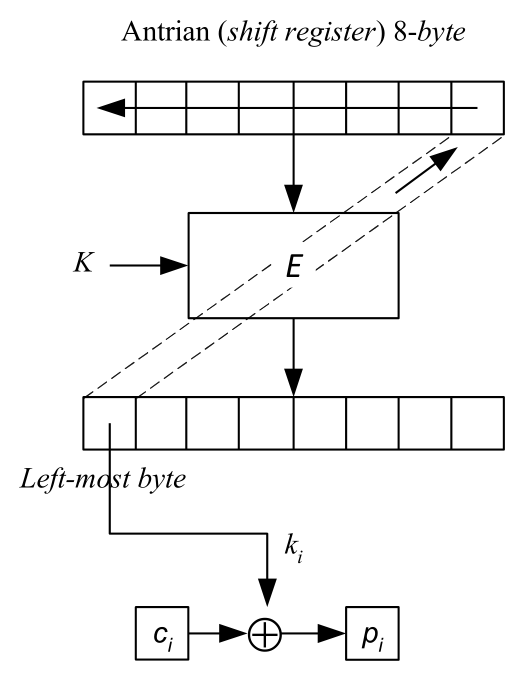
\includegraphics[width=56.70mm,height=187.11mm]{images/llm/page_042_img_02.png}%
\end{textblock*}

\newpage

% --- unit llm 43 ---
% === Halaman 43 (llm) ===

\vspace{136.62mm}

(a) Encryption
\vspace{80mm}
(b) Decryption

% deskripsi: Diagram blok proses enkripsi yang menunjukkan penggunaan shift register, blok enkripsi dengan kunci K, seleksi bit, dan operasi XOR dengan plaintext P untuk menghasilkan ciphertext C.
% bbox normalisasi: [0.1000, 0.0000, 0.9000, 0.4600]
\begin{textblock*}{168.00mm}(21.00mm,0.00mm)
\noindent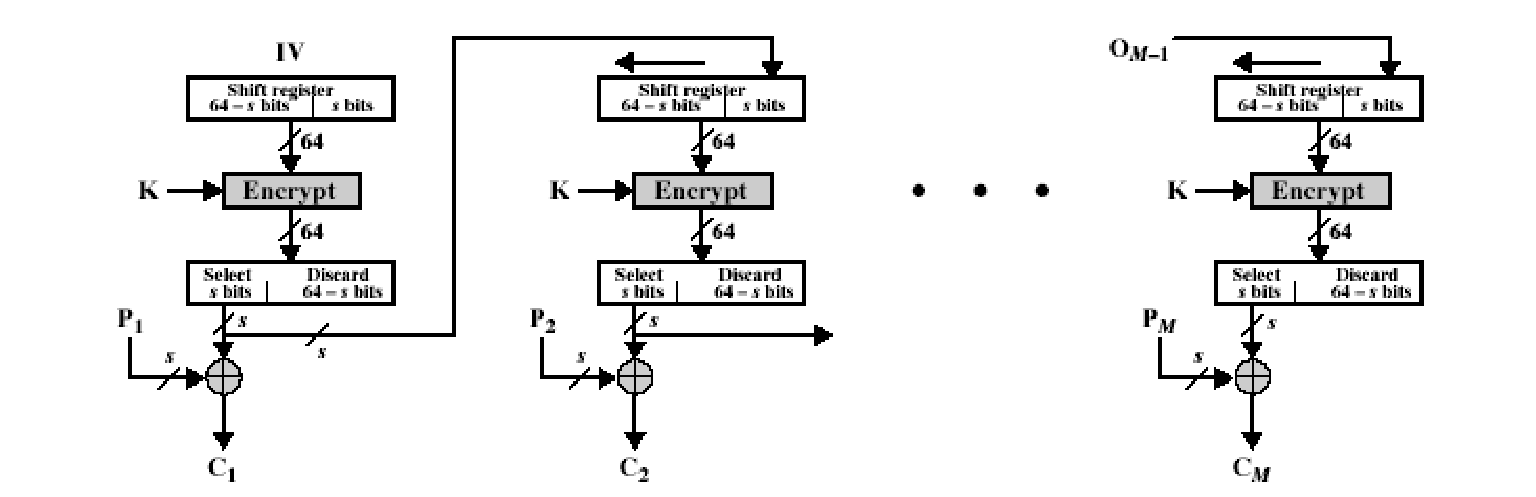
\includegraphics[width=168.00mm,height=136.62mm]{images/llm/page_043_img_01.png}%
\end{textblock*}

% deskripsi: Diagram blok proses dekripsi yang menunjukkan penggunaan shift register, blok dekripsi dengan kunci K, seleksi bit, dan operasi XOR dengan ciphertext C untuk mengembalikan plaintext P.
% bbox normalisasi: [0.1000, 0.5000, 0.9000, 0.9600]
\begin{textblock*}{168.00mm}(21.00mm,148.50mm)
\noindent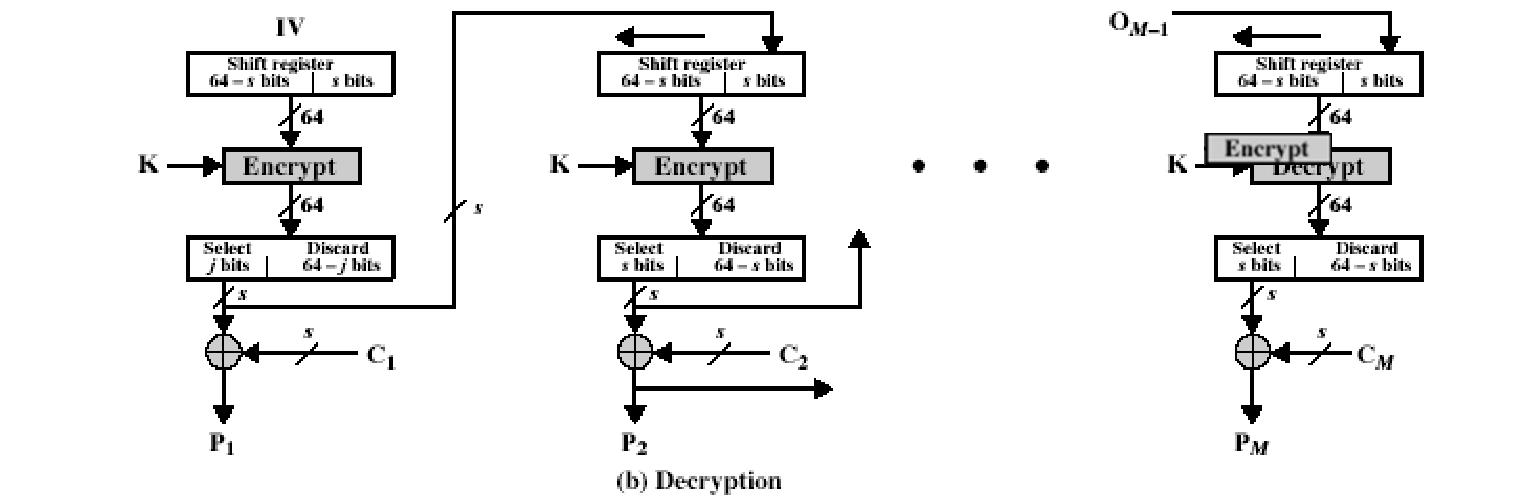
\includegraphics[width=168.00mm,height=136.62mm]{images/llm/page_043_img_02.png}%
\end{textblock*}

\newpage

% --- unit llm 44 ---
% === Halaman 44 (llm) ===

\vspace{142.56mm}

Jika $s = b$, maka mode $OFB$ $s$-bit adalah seperti pada Gambar berikut

% deskripsi: Diagram alur proses enkripsi dan dekripsi menggunakan mode Output Feedback (OFB) s-bit, yang terdiri dari dua bagian: (a) Encryption dan (b) Decryption.
% bbox normalisasi: [0.0100, 0.2800, 0.9700, 0.7600]
\begin{textblock*}{201.60mm}(2.10mm,83.16mm)
\noindent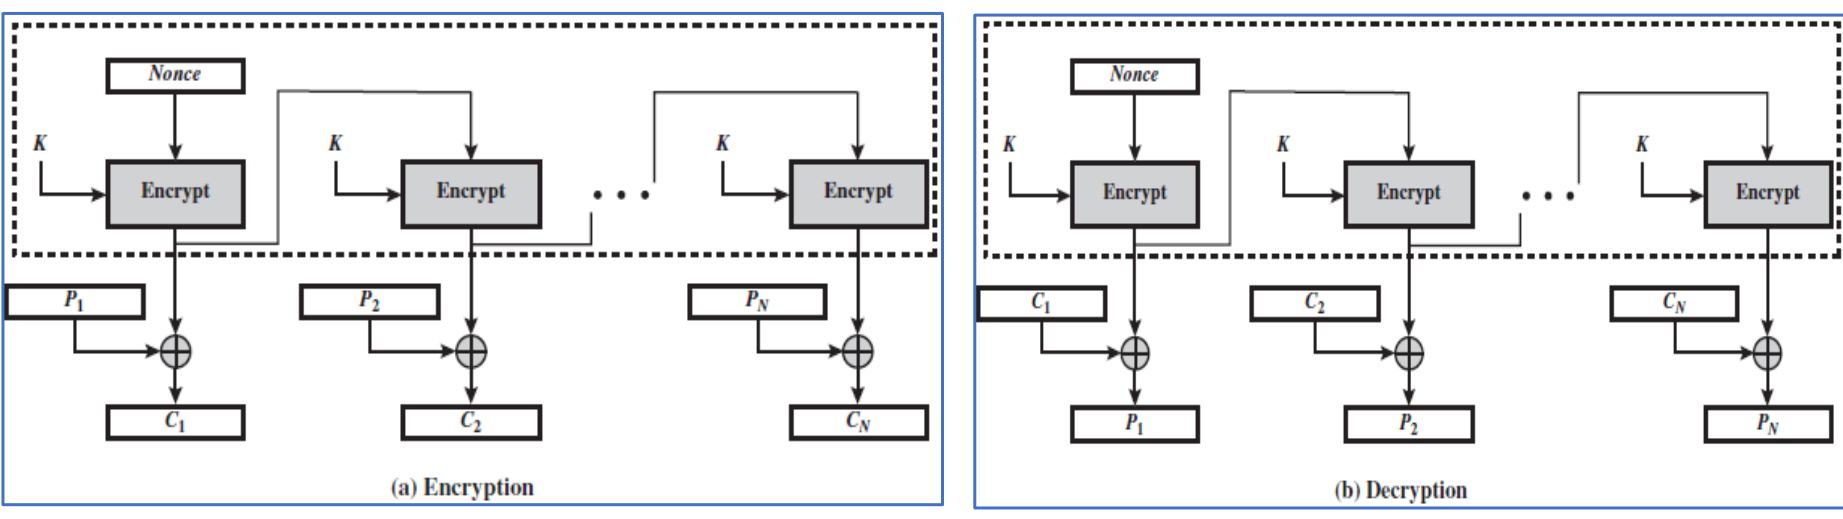
\includegraphics[width=201.60mm,height=142.56mm]{images/llm/page_044_img_01.png}%
\end{textblock*}

\newpage

% --- unit llm 45 ---
% === Halaman 45 (llm) ===

\begin{itemize}
    \item Kesalahan 1-bit pada blok plainteks hanya mempengaruhi blok cipherteks yang berkoresponden saja; begitu pula pada proses dekripsi, kesalahan 1-bit pada blok cipherteks hanya mempengaruhi blok plainteks yang bersangkutan saja.
\end{itemize}

\vspace{60mm}

\begin{itemize}
    \item Karakteristik kesalahan semacam ini cocok untuk transmisi analog yang didigitisasi, seperti suara atau video, yang dalam hal ini kesalahan 1-bit dapat ditolerir, tetapi penjalaran kesalahan tidak dibolehkan.
\end{itemize}

% deskripsi: Diagram proses enkripsi (a) dan dekripsi (b) menggunakan mode operasi cipher blok yang menunjukkan bagaimana nonce dan kunci K digunakan untuk menghasilkan cipherteks C dan plainteks P.
% bbox normalisasi: [0.0080, 0.2710, 0.9640, 0.7320]
\begin{textblock*}{200.76mm}(1.68mm,80.49mm)
\noindent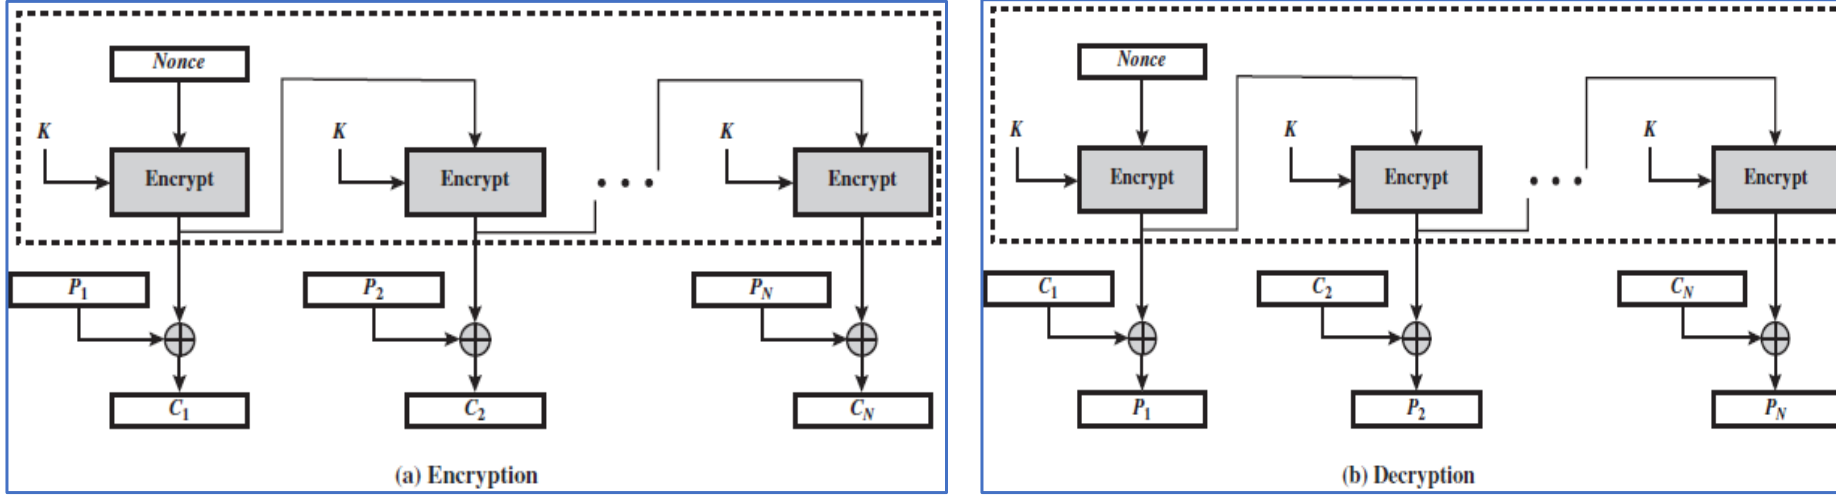
\includegraphics[width=200.76mm,height=136.92mm]{images/llm/page_045_img_01.png}%
\end{textblock*}

\newpage

% --- unit llm 46 ---
% === Halaman 46 (llm) ===

\section*{Counter Mode}

\begin{itemize}
    \item Mode \textit{counter} tidak melakukan perantaian (\textit{chaining}) seperti pada CBC.
    \item \textit{Counter} adalah sebuah nilai berupa blok bit yang ukurannya sama dengan ukuran blok plainteks.
    \item Nilai \textit{counter} harus berbeda dari setiap blok yang dienkripsi. Pada mulanya, untuk enkripsi blok pertama, \textit{counter} diinisialisasi dengan sebuah nilai.
    \item Selanjutnya, untuk enkripsi blok-blok berikutnya \textit{counter} dinaikkan (\textit{increment}) nilainya satu \[ \text{counter} \leftarrow \text{counter} + 1 ). \]

\newpage

% --- unit llm 47 ---
% === Halaman 47 (llm) ===

\vspace{68.31mm}

(a) Enkripsi
\vspace{60mm}
(b) Dekripsi

\vspace{98.01mm}

% deskripsi: Diagram alur proses enkripsi menggunakan Counter Mode (CTR), menunjukkan input Counter, Kunci (K), Plaintext (P) yang di-XOR dengan output enkripsi E untuk menghasilkan Ciphertext (C).
% bbox normalisasi: [0.2200, 0.2000, 0.8800, 0.4300]
\begin{textblock*}{138.60mm}(46.20mm,59.40mm)
\noindent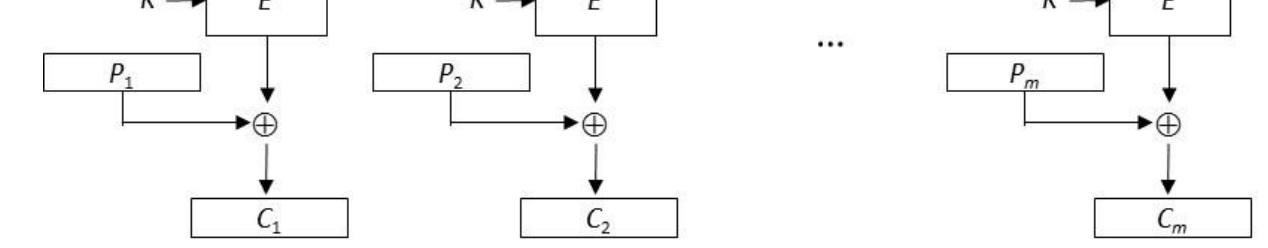
\includegraphics[width=138.60mm,height=68.31mm]{images/llm/page_047_img_01.png}%
\end{textblock*}

% deskripsi: Diagram alur proses dekripsi menggunakan Counter Mode (CTR), menunjukkan input Counter, Kunci (K), dan Ciphertext (C) yang di-XOR dengan output enkripsi E untuk mengembalikan Plaintext (P).
% bbox normalisasi: [0.2200, 0.5300, 0.8800, 0.8600]
\begin{textblock*}{138.60mm}(46.20mm,157.41mm)
\noindent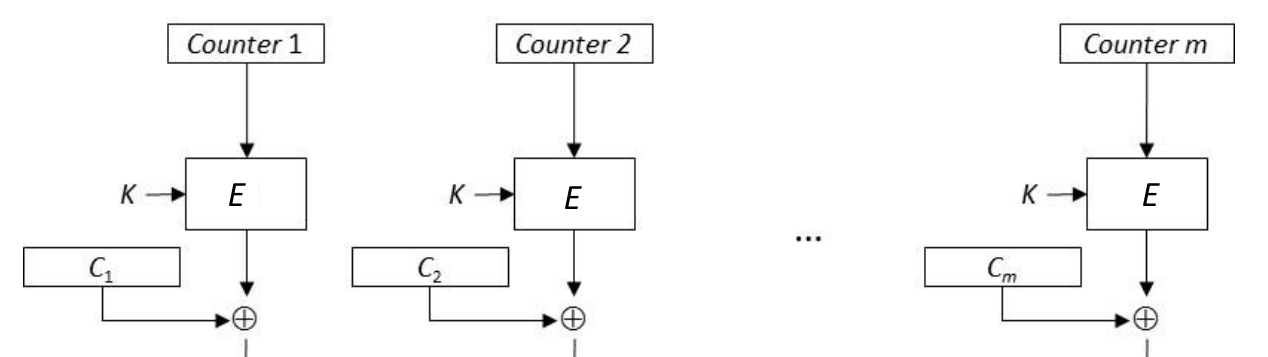
\includegraphics[width=138.60mm,height=98.01mm]{images/llm/page_047_img_02.png}%
\end{textblock*}

\newpage

% --- unit llm 48 ---
% === Halaman 48 (llm) ===

\begin{center}
\huge Mode Counter
\end{center}

\vspace{80mm}

\begin{tabular}{|l|l|}
\hline
CTR & \begin{aligned}
C_j &= P_j \oplus \text{E}(K, T_j) \quad j = 1, \dots, N-1 \\
C_N^* &= P_N^* \oplus \text{MSB}_u[\text{E}(K, T_N)]
\end{aligned} & \begin{aligned}
P_j &= C_j \oplus \text{E}(K, T_j) \quad j = 1, \dots, N-1 \\
P_N^* &= C_N^* \oplus \text{MSB}_u[\text{E}(K, T_N)]
\end{aligned} \\
\hline
\end{tabular}

\vspace{5mm}

$T_j$ adalah counter, nilainya bertambah satu untuk enkripsi blok berikutnya

% deskripsi: Diagram proses enkripsi dan dekripsi menggunakan Mode Counter (CTR), menunjukkan aliran data dari plaintext P ke ciphertext C melalui operasi XOR dengan hasil enkripsi counter.
% bbox normalisasi: [0.0000, 0.2600, 0.9900, 0.6400]
\begin{textblock*}{207.90mm}(0.00mm,77.22mm)
\noindent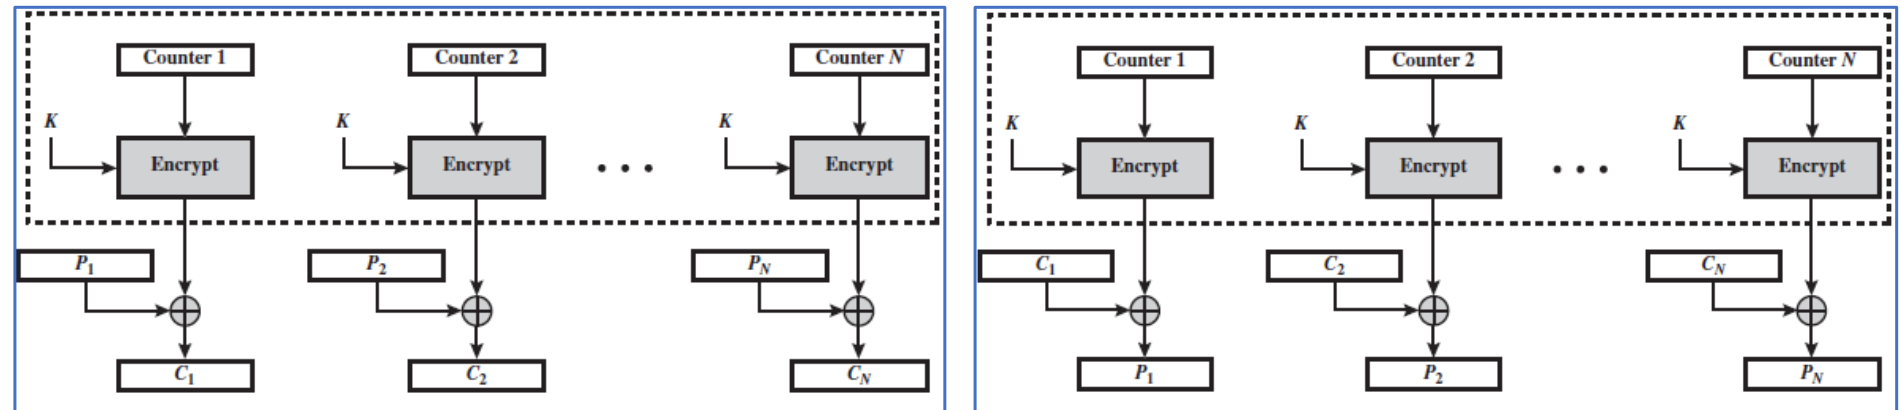
\includegraphics[width=207.90mm,height=112.86mm]{images/llm/page_048_img_01.png}%
\end{textblock*}

\newpage

% --- unit llm 49 ---
% === Halaman 49 (llm) ===

\begin{itemize}
    \item Kelebihan:
    \begin{itemize}
        \item Hanya perlu algoritma enkripsi saja
        \item Dapat mengenkripsi blok data secara acak (tidak harus sekuensial)
        \begin{itemize}
            \item Blok plainteks/cipherteks dapat diproses(enkripsi atau dekripsi) secara paralel
        \end{itemize}
        \item Sederhana, enkripsi dan dekripsi cepat
    \end{itemize}
    \vspace{10mm}
    \item Counter haruslah:
    \begin{itemize}
        \item Tidak diketahui atau tidak dapat diprediksi nilainya
    \end{itemize}
\end{itemize}

\newpage

% --- unit llm 50 ---
% === Halaman 50 (llm) ===

% (tidak ada teks dari model)

% deskripsi: Tabel yang membandingkan berbagai mode operasi cipher termasuk ECB, CBC, CFB, OFB, dan CTR, mencakup deskripsi dan aplikasi tipikal masing-masing.
% bbox normalisasi: [0.1400, 0.7000, 0.8100, 0.9030]
\begin{textblock*}{140.70mm}(29.40mm,207.90mm)
\noindent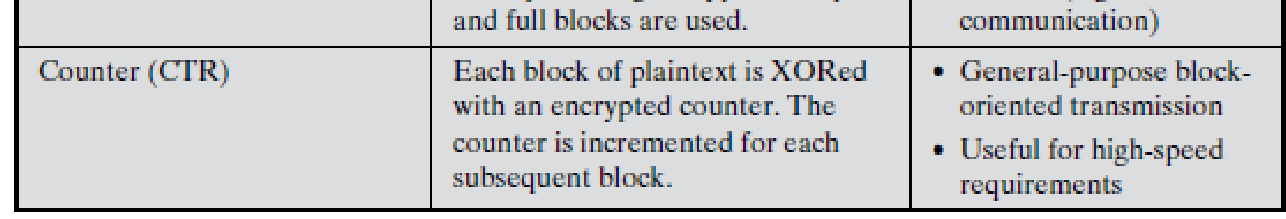
\includegraphics[width=140.70mm,height=60.29mm]{images/llm/page_050_img_01.png}%
\end{textblock*}

\newpage

% --- unit llm 51 ---
% === Halaman 51 (llm) ===

\vspace{98.90mm}

\section*{Prinsip \textit{Confusion} dan \textit{Diffusion}}

\begin{itemize}
    \item Claude Shannon dalam makalah klasiknya tahun 1949, \textit{Communication theory of secrecy systems}, memperkenalkan prinsip \textit{confusion} dan \textit{diffusion} untuk membuat serangan berbasis statistik terhadap \textit{cipher} menjadi lebih sulit dilakukan.
    \vspace{10mm}
    \item Dua prinsip tersebut, \textit{confusion} dan \textit{diffusion}, menjadi panduan dalam merancang algoritma kriptografi, baik \textit{stream cipher} maupun \textit{block cipher}.
\end{itemize}

% deskripsi: Foto potret Claude Shannon
% bbox normalisasi: [0.7930, 0.1300, 0.9260, 0.4630]
\begin{textblock*}{27.93mm}(166.53mm,38.61mm)
\noindent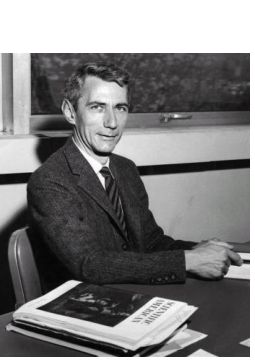
\includegraphics[width=27.93mm,height=98.90mm]{images/llm/page_051_img_01.png}%
\end{textblock*}

\newpage

% --- unit llm 52 ---
% === Halaman 52 (llm) ===

\vspace{184.14mm}

\begin{center}
\textbf{Communication Theory of Secrecy Systems$^*$}\
By C. E. SHANNON
\end{center}

\begin{center}
\textbf{1. INTRODUCTION AND SUMMARY}
\end{center}

THE problems of cryptography and secrecy systems furnish an interesting application of communication theory.$^1$ In this paper a theory of secrecy systems is developed. The approach is on a theoretical level and is intended to complement the treatment found in standard works on cryptography.$^2$ There, a detailed study is made of the many standard types of codes and ciphers, and of the ways of breaking them. We will be more concerned with the general mathematical structure and properties of secrecy systems.

The treatment is limited in certain ways. First, there are three general types of secrecy system: (1) concealment systems, including such methods as invisible ink, concealing a message in an innocent text, or in a fake covering cryptogram, or other methods in which the existence of the message is concealed from the enemy; (2) privacy systems, for example speech inversion, in which some special equipment is required to recover the message; (3) "true" secrecy systems where the meaning of the message is concealed by cipher, code, etc., although its existence is not hidden, and the enemy is assumed to have any special equipment necessary to intercept and record the transmitted signal. We consider only the third type--concealment systems are primarily a psychological problem, and privacy systems a technological one.

Secondly, the treatment is limited to the case of discrete information, where the message to be enciphered consists of a sequence of discrete symbols, each chosen from a finite set. These symbols may be letters in a language, words of a language, amplitude levels of a "quantized" speech or video signal, etc., but the main emphasis and thinking has been concerned with the case of letters.

The paper is divided into three parts. The main results will now be briefly summarized. The first part deals with the basic mathematical structure of secrecy systems. As in communication theory a language is considered to

\vspace{10mm}

\small
$^*$ The material in this paper originally appeared in a confidential report "A Mathematical Theory of Cryptography" dated Sept. 1, 1945, which has now been declassified.

$^1$ Shannon, C. E., "Communication Theory of Secrecy Systems," \textit{Bell System Technical Journal}, July 1948, p. 379; Oct. 1948, p. 625.

$^2$ See, for example, H. F. Gaines, "Elementary Cryptanalysis," or M. Givrie, "Cours de Cryptographie."

% deskripsi: Foto hitam putih Claude Shannon
% bbox normalisasi: [0.1100, 0.0300, 0.4700, 0.6500]
\begin{textblock*}{75.60mm}(23.10mm,8.91mm)
\noindent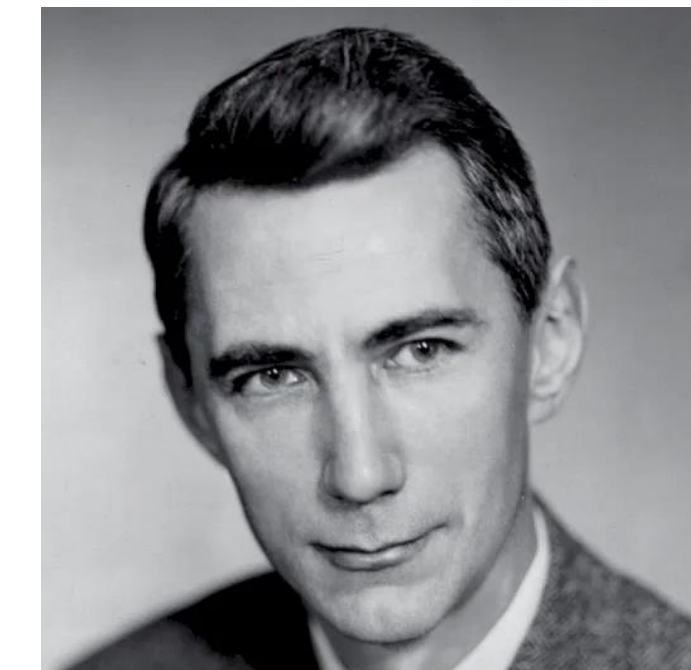
\includegraphics[width=75.60mm,height=184.14mm]{images/llm/page_052_img_01.png}%
\end{textblock*}

\newpage

% --- unit llm 53 ---
% === Halaman 53 (llm) ===

\section*{1. Confusion}

\begin{itemize}
    \item Prinsip ini menyembunyikan hubungan statistik yang ada diantara plainteks, cipherteks, dan kunci.
    \item Prinsip \textit{confusion} membuat kriptanalis frustasi untuk mencari pola-pola statistik yang muncul di dalam cipherteks.
    \item \textit{Confusion} dapat direalisasikan dengan menggunakan teknik substitusi yang nirlanjar (\textit{non-linear}), biasanya dengan operasi \textit{lookup table}.
\end{itemize}

\newpage

% --- unit llm 54 ---
% === Halaman 54 (llm) ===

\section*{Contoh substitusi di dalam $block\ cipher$ DES:}

\begin{itemize}
    \item Misalkan 6-bit masukan adalah $\mathbf{110100}$

    Substitusi 6-bit masukan dengan menggunakan tabel substitusi (S-Box). Caranya: Nomor baris tabel (bit ke-1 dan bit ke-6) = 10 (baris 2)

\vspace{62.37mm}

    Nomor kolom tabel (bit ke-2, 3, 4, dan 5) = 1010 (kolom 10)
\end{itemize}

\vspace{20mm}

Jadi, substitusi untuk 110100 adalah $entry$ pada baris 2 dan kolom 10, yaitu entri bernillai 4 atau 0100 dalam biner.

% deskripsi: Tabel S-Box DES yang menunjukkan pemetaan baris dan kolom untuk proses substitusi, dengan sel baris 2 kolom 10 yang diarsir biru.
% bbox normalisasi: [0.1400, 0.4200, 0.9200, 0.6300]
\begin{textblock*}{163.80mm}(29.40mm,124.74mm)
\noindent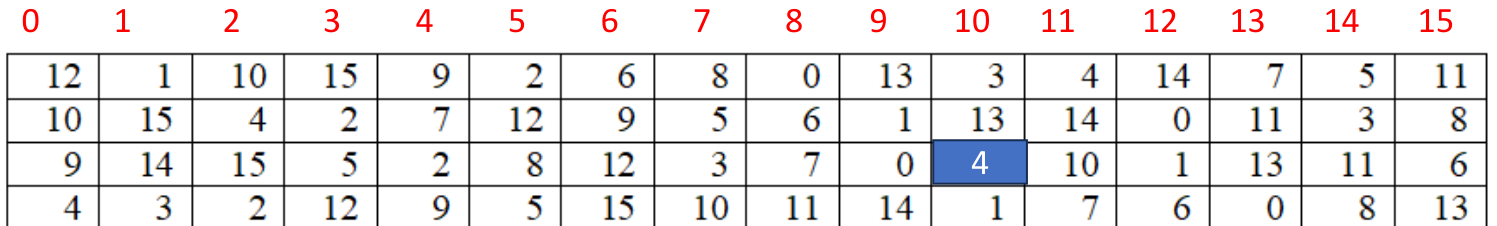
\includegraphics[width=163.80mm,height=62.37mm]{images/llm/page_054_img_01.png}%
\end{textblock*}

\newpage

% --- unit llm 55 ---
% === Halaman 55 (llm) ===

\section*{Contoh substitusi di dalam block cipher AES:}

\vspace{60mm}

\noindent Input: 23 (Hexadecimal)\\
Output: 26 (Hexadecimal)

\noindent Cara substitusi;\begin{itemize}
    \item Cari perpotongan baris 2 dengan kolom 3
    \item hasilnya adalah 26
\end{itemize}

% deskripsi: Tabel substitusi (S-Box) untuk AES yang berisi nilai-nilai hexadecimal dalam grid 16x16.
% bbox normalisasi: [0.0000, 0.1600, 0.6800, 0.7700]
\begin{textblock*}{142.80mm}(0.00mm,47.52mm)
\noindent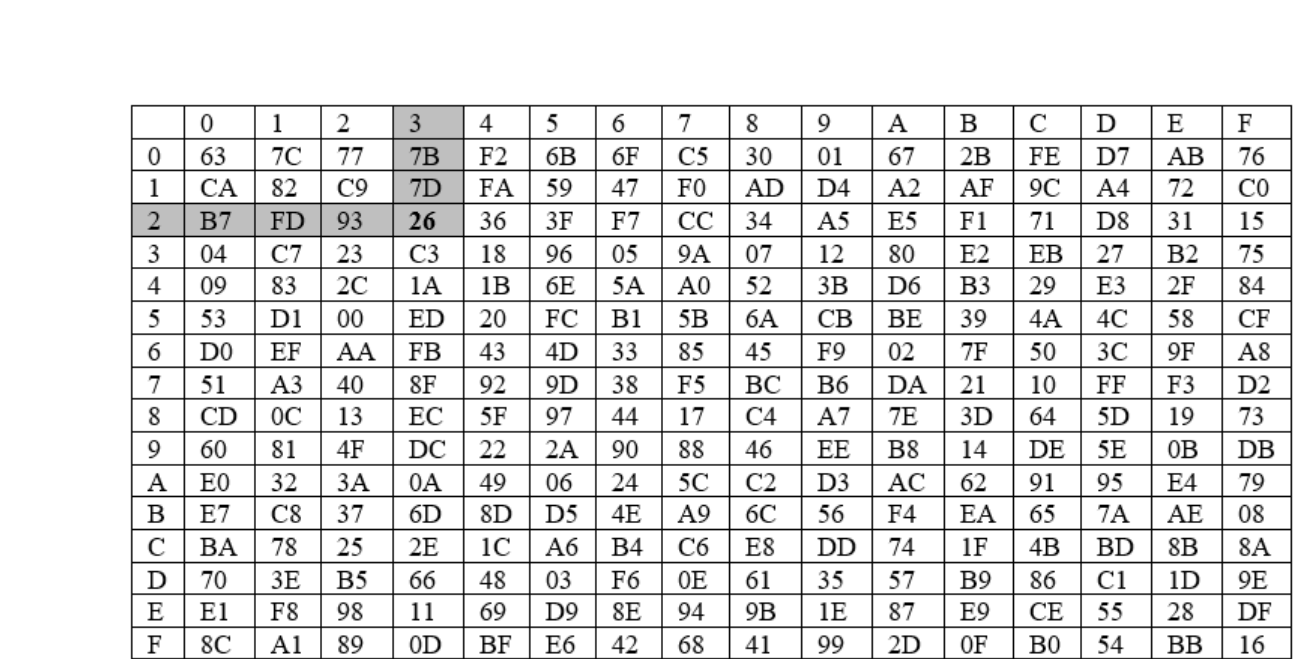
\includegraphics[width=142.80mm,height=181.17mm]{images/llm/page_055_img_01.png}%
\end{textblock*}

\newpage

% --- unit llm 56 ---
% === Halaman 56 (llm) ===

\section*{2. Diffusion}

\begin{itemize}
    \item Prinsip ini menyebarkan pengaruh satu bit plainteks atau kunci ke sebanyak mungkin bit cipherteks.
    Contoh: satu huruf plainteks mempengaruhi nilai banyak huruf cipherteks
    
    \item Sebagai efek difusi, maka pengubahan kecil pada plainteks sebanyak satu atau dua bit menghasilkan perubahan pada bit-bit cipherteks yang tidak dapat diprediksi.
    
    \item Contoh: mengenkripsi plainteks \texttt{1111111111111111} \\ 
    menghasilkan cipherteks \texttt{01101100000101001}. \\ 
    Misalkan 1 bit pertama plainteks diubah menjadi \texttt{0111111111111111}. Jika difusi bekerja, maka cipherteksnya berubah signifikan menjadi \texttt{10110010111011111}
    
    \item \textit{Diffusion} did alam block cipher dapat direalisasikan dengan menggunakan teknik permutasi atau transposisi secara berulang-ulang. Permutasi adalah mengacak susunan bit atau \textit{byte} di dalam plainteks.
\end{itemize}

\newpage

% --- unit llm 57 ---
% === Halaman 57 (llm) ===

\begin{itemize}
  \item Permutasi adalah teknik untuk mengacak susunan bit di dalam sebuah blok bit menghasilkan susunan baru.
\end{itemize}

\vspace{60mm}

\begin{itemize}
  \item Pada gambar di atas, posisi bit-bit di dalam blok input 32-bit dipermutasi menjadi susunan baru.
\end{itemize}

% deskripsi: Diagram permutasi bit yang menunjukkan pemetaan posisi dari blok input 32-bit ke posisi baru di blok output.
% bbox normalisasi: [0.1000, 0.3500, 0.8700, 0.6500]
\begin{textblock*}{161.70mm}(21.00mm,103.95mm)
\noindent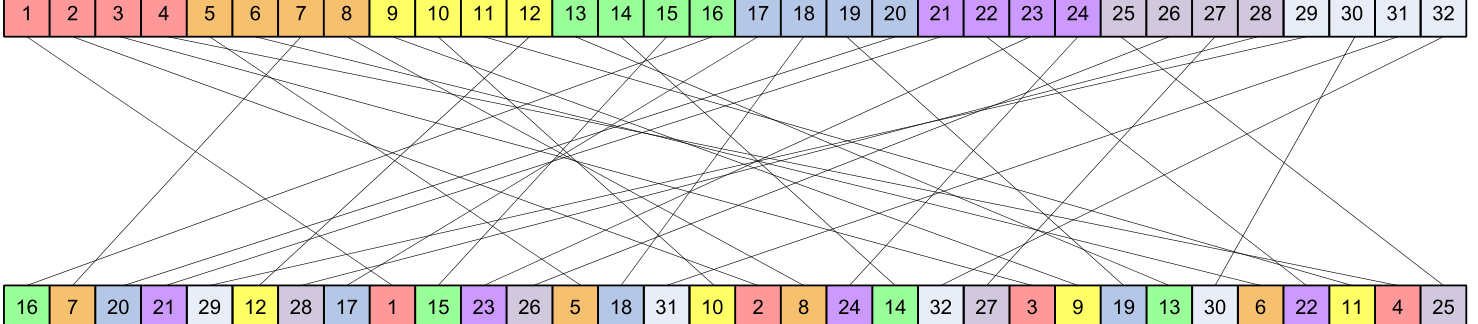
\includegraphics[width=161.70mm,height=89.10mm]{images/llm/page_057_img_01.png}%
\end{textblock*}

\newpage

% --- unit llm 58 ---
% === Halaman 58 (llm) ===

\begin{itemize}
    \item Di dalam beberapa \textit{cipher} blok, permutasi direalisasikan dengan menggunakan matriks permutasi yang dinamakan $P$-box. Entri di dalam $P$-box menyatakan bit dari posisi sebelumnya.
    \item Contoh P-box di dalam DES:
\end{itemize}

\vspace{10mm}

Artinya, bit ke 58 dari bit-bit input dipindahkan ke posisi pertama, bit ke-50 pada posisi kedua, dst

\vspace{10mm}

\begin{itemize}
    \item Beberapa skema permutasi juga melakukan kompresi (mengurangi bit-bit input) atau ekspansi (memperbanyak bit-bit) pada operasi permutasi.
\end{itemize}

% deskripsi: Tabel matriks P-box DES yang berisi angka-angka posisi bit.
% bbox normalisasi: [0.1000, 0.3100, 0.9600, 0.5100]
\begin{textblock*}{180.60mm}(21.00mm,92.07mm)
\noindent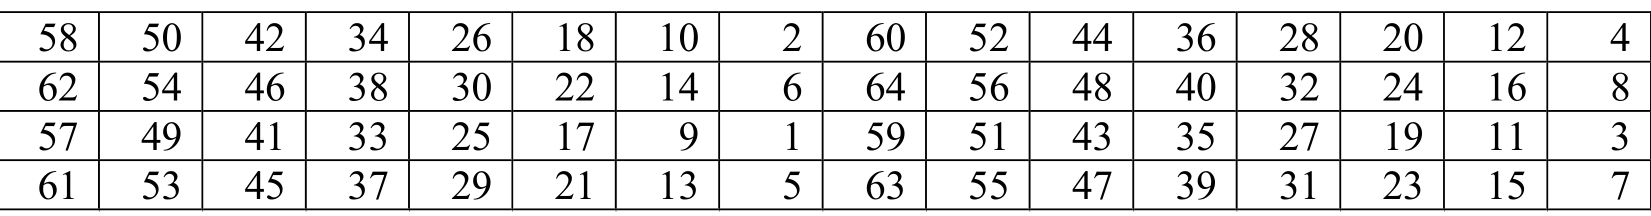
\includegraphics[width=180.60mm,height=59.40mm]{images/llm/page_058_img_01.png}%
\end{textblock*}

% deskripsi: Diagram ilustrasi proses ekspansi bit dari input 'Right Half i-1' menjadi deretan bit yang lebih panjang.
% bbox normalisasi: [0.8000, 0.7800, 0.9600, 0.9200]
\begin{textblock*}{33.60mm}(168.00mm,231.66mm)
\noindent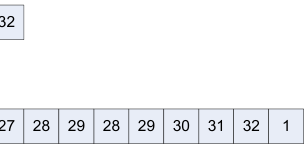
\includegraphics[width=33.60mm,height=41.58mm]{images/llm/page_058_img_02.png}%
\end{textblock*}

\newpage

% --- unit llm 59 ---
% === Halaman 59 (llm) ===

\begin{itemize}
  \item Sedangkan di dalam cipher blok yang lain, permutasi tidak menggunakan P-box, tetapi melakukan pergeseran bit ke kiri atau ke kanan sejauh k bit.
  \item Pergeseran bersifat siklik, yaitu bit yang paling ujung muncul pada ujung yang lain
  \item Contoh pergeseran byte di dalam AES:
\end{itemize}

\vspace{10mm}

% deskripsi: Diagram proses ShiftRows pada AES yang menunjukkan transformasi state menjadi state' melalui pergeseran siklik pada setiap baris.
% bbox normalisasi: [0.1220, 0.5600, 0.8770, 0.9210]
\begin{textblock*}{158.55mm}(25.62mm,166.32mm)
\noindent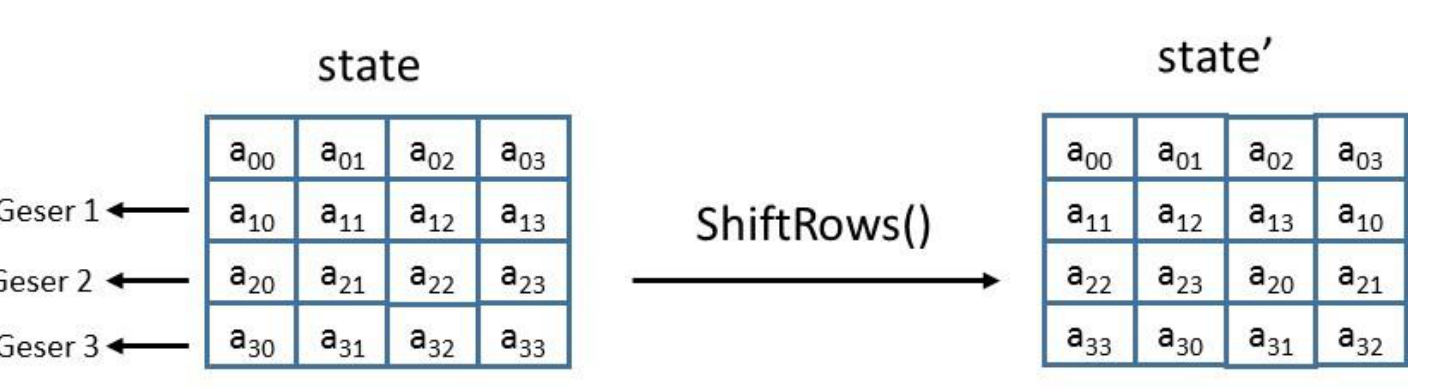
\includegraphics[width=158.55mm,height=107.22mm]{images/llm/page_059_img_01.png}%
\end{textblock*}

\newpage

% --- unit llm 60 ---
% === Halaman 60 (llm) ===

\section*{Cipher Berulang (Iterated Cipher)}

\begin{itemize}
    \item Untuk menghasilkan \textit{cipher} yang lebih kuat, maka dilakukan \textit{enciphering} sejumlah kali (sejumlah putaran) .
    \item Caranya adalah dengan melakukan berulang kali suatu fungsi transformasi $f$ (disebut juga fungsi putaran atau \textit{round function}) yang mengubah blok plainteks menjadi blokcipherteks.
    \item Pada setiap putaran digunakan upa-kunci (\textit{subkey}) atau kunci putaran (\textit{round key}) yang dikombinasikan dengan plainteks.
\end{itemize}

\vspace{10mm}

\[ i = 1, 2, ..., n \]

% deskripsi: Diagram blok yang menunjukkan proses iterasi fungsi f dengan loop balik.
% bbox normalisasi: [0.7300, 0.7300, 0.8900, 0.9300]
\begin{textblock*}{33.60mm}(153.30mm,216.81mm)
\noindent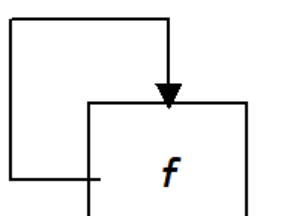
\includegraphics[width=33.60mm,height=59.40mm]{images/llm/page_060_img_01.png}%
\end{textblock*}

\newpage

% --- unit llm 61 ---
% === Halaman 61 (llm) ===

\begin{itemize}
    \item Cipher berulang dinyatakan sebagai
    \[ C_i = f(C_{i-1}, K_i) \]
    yang dalam hal ini,
    \begin{itemize}
        \item $i = 1, 2, ..., r$ ($r$ adalah jumlah putaran).
        \item $K_i$ = kunci putaran (round key) pada putaran ke-$i$
        \item $f$ = fungsi transformasi (round function), di dalamnya terdapat operasi substitusi, permutasi, dan/atau ekspansi, kompresi).
    \end{itemize}
    \item Plainteks dinyatakan dengan $C_0$ dan cipherteks dinyatakan dengan $C_r$.
\end{itemize}

\newpage

% --- unit llm 62 ---
% === Halaman 62 (llm) ===

\vspace{40mm}

$f(K_i, P)$ dinamakan fungsi putaran, $r$ adalah jumlah putaran

\textbf{DES: $r = 16$}\
\textbf{AES-128/192/256: $r = 10/12/14$}

% deskripsi: Diagram blok proses enkripsi dengan pembuatan sub-key (Sub-key generation) yang memberikan kunci $K_1, K_2, K_3, \dots, K_r$ ke dalam serangkaian fungsi putaran $f$ yang memproses input $P$ menjadi output $C$.
% bbox normalisasi: [0.1500, 0.0900, 0.9300, 0.6500]
\begin{textblock*}{163.80mm}(31.50mm,26.73mm)
\noindent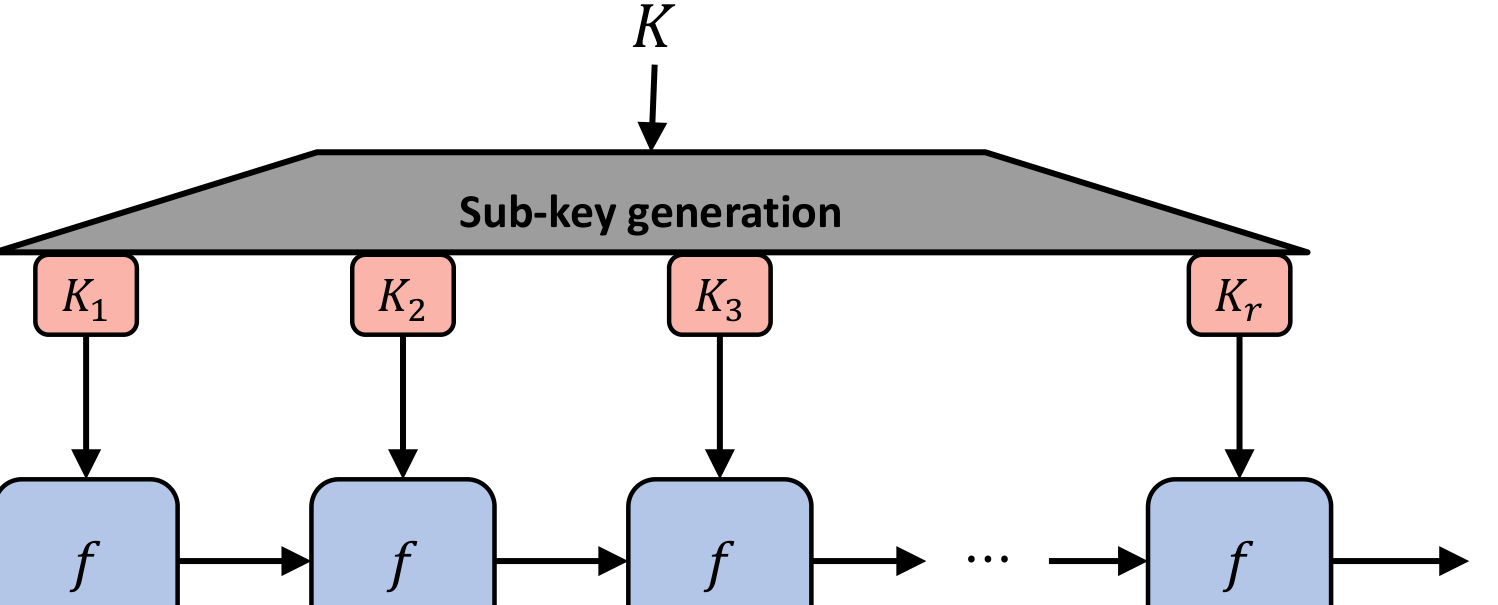
\includegraphics[width=163.80mm,height=166.32mm]{images/llm/page_062_img_01.png}%
\end{textblock*}

\newpage

% --- unit llm 63 ---
% === Halaman 63 (llm) ===

\begin{itemize}
  \item Biasanya, plainteks dimanipulasi dulu dengan kunci (umumnya di-XOR-kan dengan kunci eksternal, atau dengan kunci putaran pertama), lalu hasilnya ditransformasikan dengan fungsi $f$ berulang kali.
\end{itemize}

\vspace{10mm}

\begin{align*}
C_0 &= P \oplus K_0 \\
C_i &= f(C_{i-1}, K_i) \quad , i = 1, 2, ..., r-1 \\
C &= C_r = C_{r-1} \oplus K_r
\end{align*}

\vspace{10mm}

\begin{itemize}
  \item Semakin banyak jumlah putaran, efek diffusi semakin bertambah, namun jumlah putaran yang besar dapat memuat komputasi menjadi tidak sangkil (efisien).
  \item Jumlah putaran harus dipertimbangkan untuk mempertemukan kriteria keamanan dan efisiensi.
\end{itemize}

\newpage

% --- unit llm 64 ---
% === Halaman 64 (llm) ===

\vspace{204.93mm}

\begin{itemize}
    \item Pada setiap putaran, proses \textit{enciphering} melibatkan operasi substitusi dan permutasi. Operasi substitusi dilakukan dengan cara operasi \textit{look-up} tabel S
    \vspace{60mm}
    \item Operasi substitusi, diikuti dnegan oeprasi permutasi dilakukan pada setiap putaran. Setiap putaran menggunakan kunci putaran yang berbeda-beda ($K_1, K_2, K_3$, dst).
    \vspace{30mm}
    \item Operasi substitusi menghasilkan efek \textit{confusion}, sedangkan operasi permutasi menghasilkan efek \textit{diffusion}.
\end{itemize}

% deskripsi: Diagram alur proses enkripsi blok cipher yang menunjukkan putaran substitusi (S-box S1-S4), permutasi (P), dan operasi XOR dengan kunci putaran (K0, K1, K2, K3) mulai dari plaintext hingga menjadi ciphertext.
% bbox normalisasi: [0.5300, 0.2300, 0.9400, 0.9200]
\begin{textblock*}{86.10mm}(111.30mm,68.31mm)
\noindent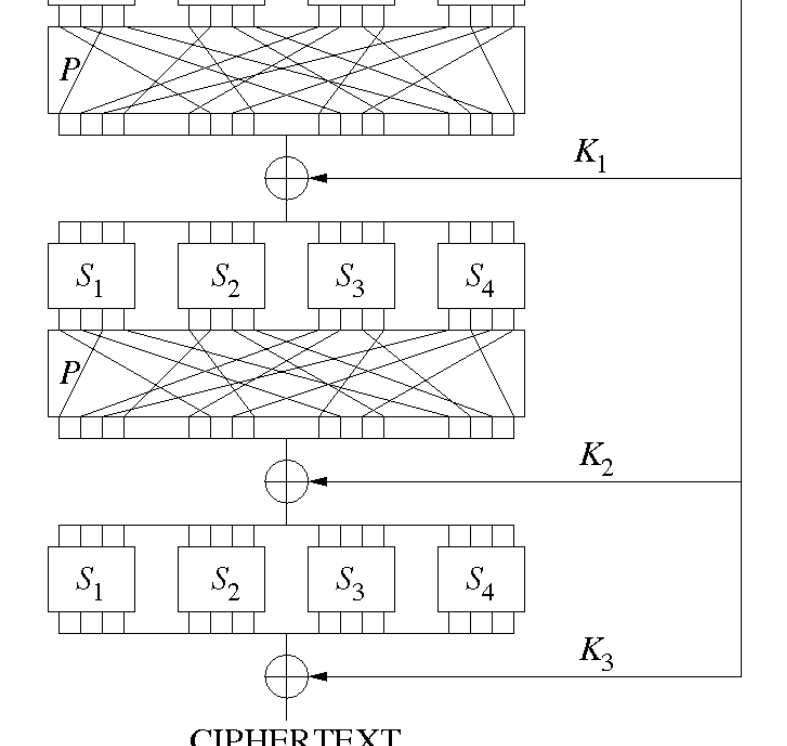
\includegraphics[width=86.10mm,height=204.93mm]{images/llm/page_064_img_01.png}%
\end{textblock*}

\newpage

% --- unit llm 65 ---
% === Halaman 65 (llm) ===

\section*{Jaringan Feistel}

\begin{itemize}
    \item Beberapa cipher blok seperti DES, GOST, Feal, Lucifer, RC5, RC6, dan lain-lain menggunakan struktur \textit{enciphering} pada setiap putaran yang dinamakan \textbf{jaringan Feistel} (\textit{Feistel Network}).
    \item Dalam hal ini, blok plainteks dibagi menjadi dua bagian, dan pada masing-masing bagian dilakukan proses transformasi menjadi upa-bagian pada putaran selanjutnya.
    \item Struktur ini bersifat \textit{reversible}, yaitu untuk melakukan dekripsi maka jaringan Feistel dieksekusi dari "bawah" ke "atas".
\end{itemize}

\newpage

% --- unit llm 66 ---
% === Halaman 66 (llm) ===

\begin{center}
\Large Feistel Network
\end{center}

\vspace{10mm}

\textbf{Encryption:}

\begin{align*}
L_1 &= R_0 & R_1 &= L_0 \oplus f_1(R_0) \\
L_2 &= R_1 & R_2 &= L_1 \oplus f_2(R_1) \\
\dots & & \dots & \\
L_i &= R_{i-1} & R_i &= L_{i-1} \oplus f_i(R_{i-1})
\end{align*}

\vspace{10mm}

\textbf{Decryption:}

\begin{align*}
R_{i-1} &= L_i & L_{i-1} &= R_i \oplus f_i(L_i) \\
\dots & & \dots & \\
R_0 &= L_1; & L_0 &= R_1 \oplus f_1(L_1)
\end{align*}

\vspace{10mm}
Sumber: Cryptography CS 555

% deskripsi: Diagram alir struktur Feistel Network untuk proses enkripsi yang menunjukkan operasi XOR dan fungsi f pada blok L dan R.
% bbox normalisasi: [0.1300, 0.1400, 0.5300, 0.5400]
\begin{textblock*}{84.00mm}(27.30mm,41.58mm)
\noindent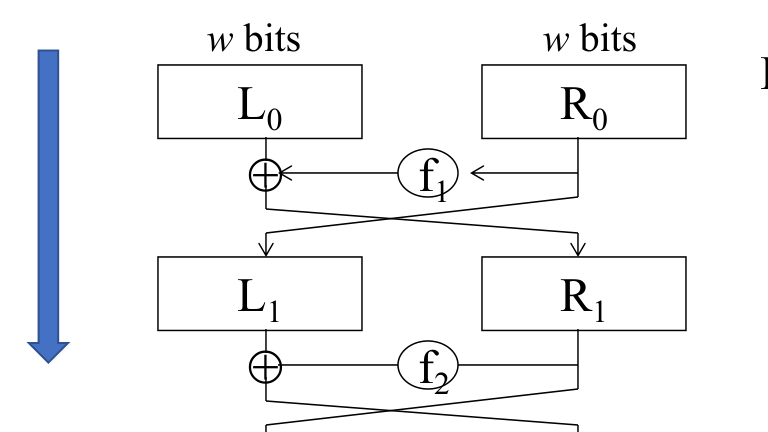
\includegraphics[width=84.00mm,height=118.80mm]{images/llm/page_066_img_01.png}%
\end{textblock*}

% deskripsi: Diagram alir struktur Feistel Network untuk proses dekripsi yang menunjukkan pembalikan operasi blok L dan R.
% bbox normalisasi: [0.1200, 0.6700, 0.5300, 0.9200]
\begin{textblock*}{86.10mm}(25.20mm,198.99mm)
\noindent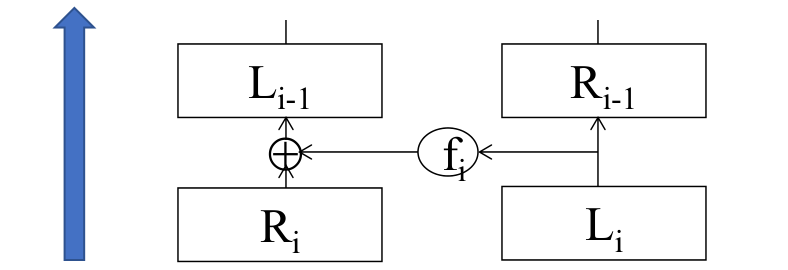
\includegraphics[width=86.10mm,height=74.25mm]{images/llm/page_066_img_02.png}%
\end{textblock*}

\newpage

% --- unit llm 67 ---
% === Halaman 67 (llm) ===

\vspace{160.38mm}

Contoh jaringan Feistel di dalam DES:\
\vspace{60mm}
Jaringan $Feistel$ pada enkripsi putaran ke-$i$
\[ 
\begin{aligned}
L_i &= R_{i-1} \\
R_i &= L_{i-1} \oplus f(R_{i-1}, K_i)
\end{aligned}
\]

% deskripsi: Diagram alir jaringan Feistel yang menunjukkan proses transformasi data antara L dan R menggunakan fungsi f dan kunci Ki.
% bbox normalisasi: [0.1400, 0.2300, 0.8200, 0.7700]
\begin{textblock*}{142.80mm}(29.40mm,68.31mm)
\noindent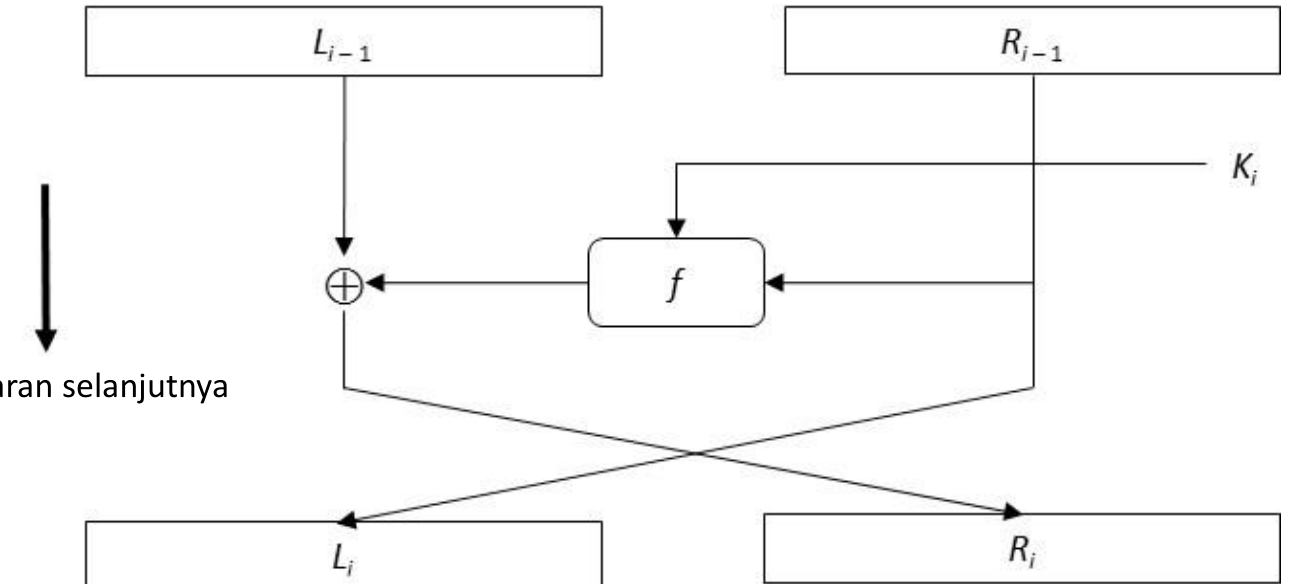
\includegraphics[width=142.80mm,height=160.38mm]{images/llm/page_067_img_01.png}%
\end{textblock*}

\newpage

% --- unit llm 68 ---
% === Halaman 68 (llm) ===

\begin{itemize}
  \item Untuk melakukan dekripsi, maka urutan komputasi di dalam Feistel dibalik (dari "bawah" ke "atas"), itulah sebabnya dinamakan \textit{reversible}.
\end{itemize}

\vspace{60mm}

Jaringan \textit{Feistel} pada dekripsi putaran ke-$i$

\begin{align*}
  R_{i-1} &= L_i \\
  L_{i-1} &= R_i \oplus f(R_{i-1}, K_i) = R_i \oplus f(L_i, K_i)
\end{align*}

% deskripsi: Diagram alur jaringan Feistel untuk proses dekripsi putaran ke-i, menunjukkan aliran data dari L_i dan R_i kembali ke L_{i-1} dan R_{i-1} dengan fungsi f dan kunci K_i.
% bbox normalisasi: [0.1180, 0.2530, 0.8100, 0.7450]
\begin{textblock*}{145.32mm}(24.78mm,75.14mm)
\noindent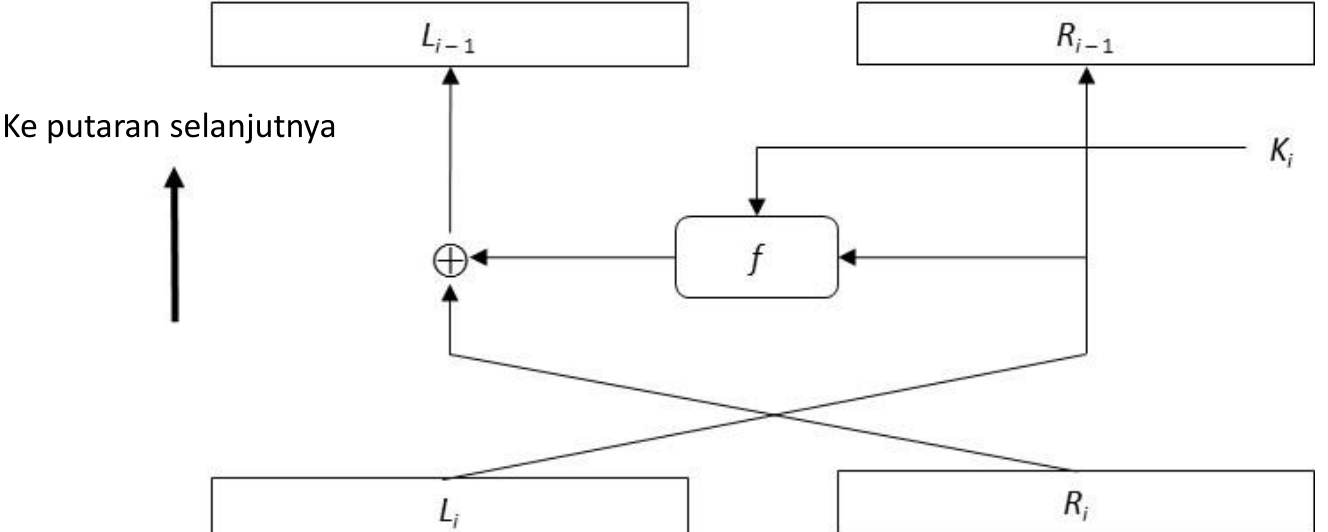
\includegraphics[width=145.32mm,height=146.12mm]{images/llm/page_068_img_01.png}%
\end{textblock*}

\newpage

% --- unit llm 69 ---
% === Halaman 69 (llm) ===

\begin{itemize}
  \item Sifat \textit{reversible} ini membuat perancang cipher blok tidak perlu membuat algoritma baru untuk mendekripsi cipherteks menjadi plainteks.

  Contoh: \[ L_{i-1} \oplus f(R_{i-1}, K_i) \oplus f(R_{i-1}, K_i) = L_{i-1} \]

  \item Sifat \textit{reversible} tidak bergantung pada fungsi $f$ sehingga fungsi $f$ dapat dibuat serumit mungkin.
\end{itemize}

\newpage

% --- unit llm 70 ---
% === Halaman 70 (llm) ===

\section*{Pembangkitan kunci putaran}

\begin{itemize}
    \item Setiap putaran di dalam \textit{iterated cipher} menggunakan kunci internal (\textit{subkey}) yang dinamakan kunci putaran (\textit{round key}).
    \item Kunci putaran dibangkitkan dari kunci eksternal yang diberikan oleh \textit{user} melalui proses yang dinamakan \textit{key expansion} atau \textit{key scheduling}.
    \item Di dalam \textit{key expansion} dilakukan komputasi yang kompleks untuk menghasilkan sejumlah kunci putaran yang berbeda-beda.
    \item Panjang kunci putaran tidak selalu sama dengan panjang kunci eksternal.
\end{itemize}

\newpage

% --- unit llm 71 ---
% === Halaman 71 (llm) ===

\vspace{240.57mm}

\textbf{Gambar} pembangkitan kunci putaran di dalam DES

% deskripsi: Diagram alir proses pembangkitan kunci putaran (key scheduling) dalam algoritma DES, menunjukkan transformasi dari Kunci eksternal 64 bit melalui Permutasi PC-1, pemisahan menjadi C dan D masing-masing 28 bit, operasi Left Shift berulang, dan Permutasi PC-2 untuk menghasilkan kunci sub-kunci $K_1, K_j,$ hingga $K_{16}$ yang masing-masing berukuran 48 bit.
% bbox normalisasi: [0.0400, 0.1500, 0.6500, 0.9600]
\begin{textblock*}{128.10mm}(8.40mm,44.55mm)
\noindent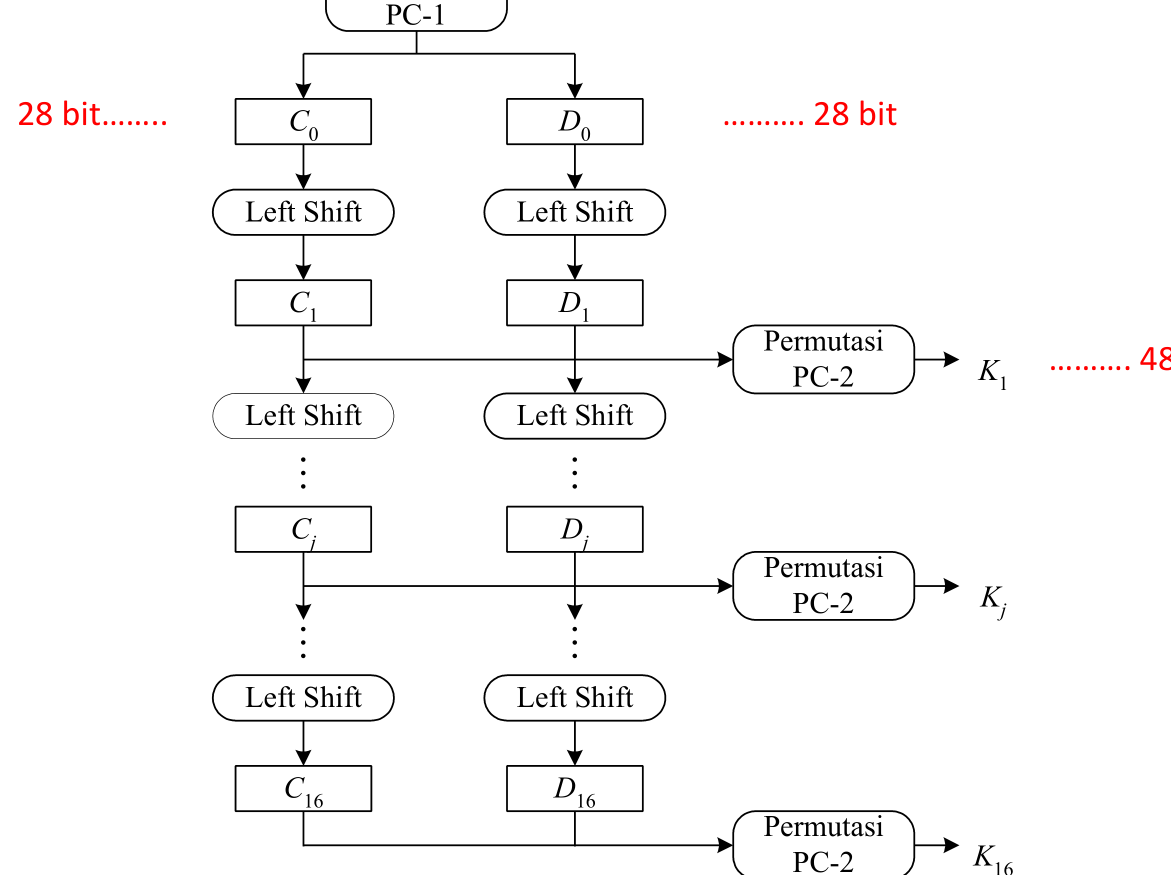
\includegraphics[width=128.10mm,height=240.57mm]{images/llm/page_071_img_01.png}%
\end{textblock*}

\newpage

% --- unit llm 72 ---
% === Halaman 72 (llm) ===

\section*{Ukuran blok dan kunci}

\begin{itemize}
    \item Ukuran blok pesan ($n$) yang diproses selama enkripsi/dekripsi selalu tetap.
    
    Contoh: DES ($n = 64$), AES ($n = 128, 192, 256$)
    
    \item Makin besar ukuran blok mengarah ke efek \textit{diffusion} yang lebih besar.
    
    \item Ukuran kunci ($m$) bisa sama dengan ukuran blok atau berbeda dengan ukuran blok
    
    Contoh: DES ($m = 56$), AES ($m = 128, 192, 256$)
    
    \item Makin besar ukuran kunci mengarah ke efek \textit{confusion} yang lebih besar dan lebih tahan terhadap serangan \textit{brute force}.
\end{itemize}

\newpage

% --- unit llm 73 ---
% === Halaman 73 (llm) ===

Bersambung

\newpage

% --- unit llm 74 ---
% === Halaman 74 (llm) ===

Bersambung

\end{document}
